\documentclass[]{book}
\usepackage{lmodern}
\usepackage{amssymb,amsmath}
\usepackage{ifxetex,ifluatex}
\usepackage{fixltx2e} % provides \textsubscript
\ifnum 0\ifxetex 1\fi\ifluatex 1\fi=0 % if pdftex
  \usepackage[T1]{fontenc}
  \usepackage[utf8]{inputenc}
\else % if luatex or xelatex
  \ifxetex
    \usepackage{mathspec}
  \else
    \usepackage{fontspec}
  \fi
  \defaultfontfeatures{Ligatures=TeX,Scale=MatchLowercase}
\fi
% use upquote if available, for straight quotes in verbatim environments
\IfFileExists{upquote.sty}{\usepackage{upquote}}{}
% use microtype if available
\IfFileExists{microtype.sty}{%
\usepackage{microtype}
\UseMicrotypeSet[protrusion]{basicmath} % disable protrusion for tt fonts
}{}
\usepackage[margin=1in]{geometry}
\usepackage{hyperref}
\hypersetup{unicode=true,
            pdftitle={Statistique Inférentielle},
            pdfauthor={Mohamad Ghassany},
            pdfborder={0 0 0},
            breaklinks=true}
\urlstyle{same}  % don't use monospace font for urls
\usepackage{natbib}
\bibliographystyle{apalike}
\usepackage{color}
\usepackage{fancyvrb}
\newcommand{\VerbBar}{|}
\newcommand{\VERB}{\Verb[commandchars=\\\{\}]}
\DefineVerbatimEnvironment{Highlighting}{Verbatim}{commandchars=\\\{\}}
% Add ',fontsize=\small' for more characters per line
\usepackage{framed}
\definecolor{shadecolor}{RGB}{248,248,248}
\newenvironment{Shaded}{\begin{snugshade}}{\end{snugshade}}
\newcommand{\AlertTok}[1]{\textcolor[rgb]{0.94,0.16,0.16}{#1}}
\newcommand{\AnnotationTok}[1]{\textcolor[rgb]{0.56,0.35,0.01}{\textbf{\textit{#1}}}}
\newcommand{\AttributeTok}[1]{\textcolor[rgb]{0.77,0.63,0.00}{#1}}
\newcommand{\BaseNTok}[1]{\textcolor[rgb]{0.00,0.00,0.81}{#1}}
\newcommand{\BuiltInTok}[1]{#1}
\newcommand{\CharTok}[1]{\textcolor[rgb]{0.31,0.60,0.02}{#1}}
\newcommand{\CommentTok}[1]{\textcolor[rgb]{0.56,0.35,0.01}{\textit{#1}}}
\newcommand{\CommentVarTok}[1]{\textcolor[rgb]{0.56,0.35,0.01}{\textbf{\textit{#1}}}}
\newcommand{\ConstantTok}[1]{\textcolor[rgb]{0.00,0.00,0.00}{#1}}
\newcommand{\ControlFlowTok}[1]{\textcolor[rgb]{0.13,0.29,0.53}{\textbf{#1}}}
\newcommand{\DataTypeTok}[1]{\textcolor[rgb]{0.13,0.29,0.53}{#1}}
\newcommand{\DecValTok}[1]{\textcolor[rgb]{0.00,0.00,0.81}{#1}}
\newcommand{\DocumentationTok}[1]{\textcolor[rgb]{0.56,0.35,0.01}{\textbf{\textit{#1}}}}
\newcommand{\ErrorTok}[1]{\textcolor[rgb]{0.64,0.00,0.00}{\textbf{#1}}}
\newcommand{\ExtensionTok}[1]{#1}
\newcommand{\FloatTok}[1]{\textcolor[rgb]{0.00,0.00,0.81}{#1}}
\newcommand{\FunctionTok}[1]{\textcolor[rgb]{0.00,0.00,0.00}{#1}}
\newcommand{\ImportTok}[1]{#1}
\newcommand{\InformationTok}[1]{\textcolor[rgb]{0.56,0.35,0.01}{\textbf{\textit{#1}}}}
\newcommand{\KeywordTok}[1]{\textcolor[rgb]{0.13,0.29,0.53}{\textbf{#1}}}
\newcommand{\NormalTok}[1]{#1}
\newcommand{\OperatorTok}[1]{\textcolor[rgb]{0.81,0.36,0.00}{\textbf{#1}}}
\newcommand{\OtherTok}[1]{\textcolor[rgb]{0.56,0.35,0.01}{#1}}
\newcommand{\PreprocessorTok}[1]{\textcolor[rgb]{0.56,0.35,0.01}{\textit{#1}}}
\newcommand{\RegionMarkerTok}[1]{#1}
\newcommand{\SpecialCharTok}[1]{\textcolor[rgb]{0.00,0.00,0.00}{#1}}
\newcommand{\SpecialStringTok}[1]{\textcolor[rgb]{0.31,0.60,0.02}{#1}}
\newcommand{\StringTok}[1]{\textcolor[rgb]{0.31,0.60,0.02}{#1}}
\newcommand{\VariableTok}[1]{\textcolor[rgb]{0.00,0.00,0.00}{#1}}
\newcommand{\VerbatimStringTok}[1]{\textcolor[rgb]{0.31,0.60,0.02}{#1}}
\newcommand{\WarningTok}[1]{\textcolor[rgb]{0.56,0.35,0.01}{\textbf{\textit{#1}}}}
\usepackage{longtable,booktabs}
\usepackage{graphicx,grffile}
\makeatletter
\def\maxwidth{\ifdim\Gin@nat@width>\linewidth\linewidth\else\Gin@nat@width\fi}
\def\maxheight{\ifdim\Gin@nat@height>\textheight\textheight\else\Gin@nat@height\fi}
\makeatother
% Scale images if necessary, so that they will not overflow the page
% margins by default, and it is still possible to overwrite the defaults
% using explicit options in \includegraphics[width, height, ...]{}
\setkeys{Gin}{width=\maxwidth,height=\maxheight,keepaspectratio}
\IfFileExists{parskip.sty}{%
\usepackage{parskip}
}{% else
\setlength{\parindent}{0pt}
\setlength{\parskip}{6pt plus 2pt minus 1pt}
}
\setlength{\emergencystretch}{3em}  % prevent overfull lines
\providecommand{\tightlist}{%
  \setlength{\itemsep}{0pt}\setlength{\parskip}{0pt}}
\setcounter{secnumdepth}{5}
% Redefines (sub)paragraphs to behave more like sections
\ifx\paragraph\undefined\else
\let\oldparagraph\paragraph
\renewcommand{\paragraph}[1]{\oldparagraph{#1}\mbox{}}
\fi
\ifx\subparagraph\undefined\else
\let\oldsubparagraph\subparagraph
\renewcommand{\subparagraph}[1]{\oldsubparagraph{#1}\mbox{}}
\fi

%%% Use protect on footnotes to avoid problems with footnotes in titles
\let\rmarkdownfootnote\footnote%
\def\footnote{\protect\rmarkdownfootnote}

%%% Change title format to be more compact
\usepackage{titling}

% Create subtitle command for use in maketitle
\providecommand{\subtitle}[1]{
  \posttitle{
    \begin{center}\large#1\end{center}
    }
}

\setlength{\droptitle}{-2em}

  \title{Statistique Inférentielle}
    \pretitle{\vspace{\droptitle}\centering\huge}
  \posttitle{\par}
    \author{Mohamad Ghassany}
    \preauthor{\centering\large\emph}
  \postauthor{\par}
      \predate{\centering\large\emph}
  \postdate{\par}
    \date{2019-06-20}

% \defaultfontfeatures{
%     Path = /home/ghassany/texmf/fonts/opentype/public/fontawesome/}
\usepackage{fontawesome}

\usepackage{booktabs}
\usepackage{longtable}
\usepackage{framed,color}
\usepackage{float}
\let\origfigure\figure
\let\endorigfigure\endfigure
\renewenvironment{figure}[1][2] {
    \expandafter\origfigure\expandafter[H]
} {
    \endorigfigure
}

\definecolor{shadecolor}{RGB}{248,248,248}

\ifxetex
  \usepackage{letltxmacro}
  \setlength{\XeTeXLinkMargin}{1pt}
  \LetLtxMacro\SavedIncludeGraphics\includegraphics
  \def\includegraphics#1#{% #1 catches optional stuff (star/opt. arg.)
    \IncludeGraphicsAux{#1}%
  }%
  \newcommand*{\IncludeGraphicsAux}[2]{%
    \XeTeXLinkBox{%
      \SavedIncludeGraphics#1{#2}%
    }%
  }%
\fi

\newenvironment{rmdblock}[1]
  {\begin{shaded*}
  \begin{itemize}
  \renewcommand{\labelitemi}{
    \raisebox{-.7\height}[0pt][0pt]{
      {\setkeys{Gin}{width=2em,keepaspectratio}\includegraphics{img/icons/#1}}
    }
  }
  \item
  }
  {
  \end{itemize}
  \end{shaded*}
  }
\newenvironment{rmdcaution}
  {\begin{rmdblock}{caution}}
  {\end{rmdblock}}
\newenvironment{rmdinsight}
  {\begin{rmdblock}{insight}}
  {\end{rmdblock}}
\newenvironment{rmdexercise}
  {\begin{rmdblock}{exercise}}
  {\end{rmdblock}}
\newenvironment{rmdtip}
  {\begin{rmdblock}{tip}}
  {\end{rmdblock}}
\newenvironment{rmdnoicon}
  {\begin{rmdblock}}
  {\end{rmdblock}}


\usepackage{color}
\usepackage[dvipsnames]{xcolor}

\makeatletter
\renewcommand{\title}[1]{\renewcommand{\@title}{\color{\@titlecolor}#1}}
\newcommand{\@titlecolor}{ForestGreen}
\newcommand{\titlecolor}[1]{\renewcommand{\@titlecolor}{#1}}
\renewcommand{\author}[1]{\renewcommand{\@author}{\color{\@authorcolor}#1}}
\newcommand{\@authorcolor}{RoyalBlue}
\newcommand{\authorcolor}[1]{\renewcommand{\@authorcolor}{#1}}
\renewcommand\section{\@startsection {section}{1}{\z@}%
                                   {-3.5ex \@plus -1ex \@minus -.2ex}%
                                   {2.3ex \@plus.2ex}%
                                   {\normalfont\Large\bfseries\color{ForestGreen}}}
\renewcommand\subsection{\@startsection{subsection}{2}{\z@}%
                                     {-3.25ex\@plus -1ex \@minus -.2ex}%
                                     {1.5ex \@plus .2ex}%
                                     {\normalfont\large\bfseries\color{Violet}}}
\renewcommand\subsubsection{\@startsection{subsubsection}{3}{\z@}%
                                     {-3.25ex\@plus -1ex \@minus -.2ex}%
                                     {1.5ex \@plus .2ex}%
                                     {\normalfont\normalsize\bfseries\color{Violet}}}
\makeatother


\newcommand{\lt}{<}
\newcommand{\gt}{>}



% NEWWW


\usepackage{lmodern}
\usepackage{amssymb,amsmath,amsthm}
\usepackage{bbm} % pour fonction indicatrice \mathbbm{1}
\usepackage{ifxetex,ifluatex}
\usepackage{color}
\usepackage[dvipsnames]{xcolor}

\usepackage[margin=1in]{geometry}

\usepackage{float}


\usepackage{booktabs}

% \newtheoremstyle{stylename}% name of the style to be used
%   {spaceabove}% measure of space to leave above the theorem. E.g.: 3pt
%   {spacebelow}% measure of space to leave below the theorem. E.g.: 3pt
%   {bodyfont}% name of font to use in the body of the theorem
%   {indent}% measure of space to indent
%   {headfont}% name of head font
%   {headpunctuation}% punctuation between head and body
%   {headspace}% space after theorem head; " " = normal interword space
%   {headspec}% Manually specify head

\newtheoremstyle{magentacolor}
  {5pt}
  {5pt}
  {\itshape}
  {}
  {\color{Magenta}\bfseries}
  {}
  { }
  {}

% \theoremstyle{plain}
\theoremstyle{magentacolor}
\newtheorem{theom}{Théorème}  
% \theoremstyle{magentacolor} 
\newtheorem{prop}[theom]{Proposition} 
% \newtheorem*{solution}{Solution}
% \theoremstyle{definition}
\newtheorem{defi}{\textcolor{magenta}{Définition}}[section]
\newtheorem*{preuve}{Démonstration}
\newtheorem*{sol}{\textcolor{PineGreen}{Solution}}
\newtheorem*{re}{\textcolor{red}{Remarque}}
\newtheoremstyle{proprie}{3pt}{3pt}{}{}{\color{RoyalBlue}\bfseries}{}{ }{}
\theoremstyle{proprie}
\newtheorem*{propriete}{Propriétés}


\newtheoremstyle{exstyle}
  {5pt} % Space above
  {5pt} % Space below
  {} % Body font
  {} % Indent amount
  {\color{Turquoise}\bfseries} % Theorem head font
  {} % Punctuation after theorem head
  {.5em} % Space after theorem head
  {} % Theorem head spec (can be left empty, meaning `normal')

\theoremstyle{exstyle}
\newtheorem{ex}{Exemple}[section] 

\newtheoremstyle{exostyle}
  {15pt} % Space above
  {15pt} % Space below
  {} % Body font
  {} % Indent amount
  {\color{ForestGreen}\bfseries} % Theorem head font
  {} % Punctuation after theorem head
  {.5em} % Space after theorem head
  {} % Theorem head spec (can be left empty, meaning `normal')

\theoremstyle{exostyle}
\newtheorem{exo}{Exercice}


\usepackage{mdframed}
% \newmdenv[skipabove=7pt,
% skipbelow=7pt,
% backgroundcolor=black!3,
% linecolor=black,
% innerleftmargin=5pt,
% innerrightmargin=5pt,
% innertopmargin=5pt,
% leftmargin=0cm,
% rightmargin=0cm,
% innerbottommargin=5pt]{dBox}

\newmdenv[skipabove=10pt,
 skipbelow=10pt,
 frametitleaboveskip=7pt,
 frametitlebelowskip=7pt,
 backgroundcolor=gray!4,
 frametitlerule=false,
 frametitlebackgroundcolor=black!20,
 linewidth=0pt,
 innerleftmargin=5pt,
innerrightmargin=5pt,
innertopmargin=7pt,
innerbottommargin=7pt]{dBox}
% linecolor=black,
% innerleftmargin=5pt,
% innerrightmargin=5pt,
% innertopmargin=5pt,
% leftmargin=0cm,
% rightmargin=0cm,
% innerbottommargin=5pt]{dBox}

\newmdenv[skipabove=10pt,
 skipbelow=10pt,
 frametitleaboveskip=7pt,
 frametitlebelowskip=7pt,
 backgroundcolor=gray!4,
 frametitlerule=false,
 frametitlebackgroundcolor=black!20,
 linewidth=0pt,
 innerleftmargin=5pt,
innerrightmargin=5pt,
innertopmargin=7pt,
innerbottommargin=7pt]{dBoxPropr}

\newenvironment{de}{\begin{dBox}\begin{defi}}{\end{defi}\end{dBox}} 

\newenvironment{propr}{\begin{dBoxPropr}\begin{propriete}}{\end{propriete}\end{dBoxPropr}} 

\newenvironment{theo}{\begin{dBoxPropr}\begin{theom}}{\end{theom}\end{dBoxPropr}} 
% \newenvironment{propr}{\begin{propriete}}{\end{propriete}}

\usepackage{amsthm}
\newtheorem{theorem}{Théorème}[chapter]
\newtheorem{lemma}{Lemme}[chapter]
\newtheorem{corollary}{Corollaire}[chapter]
\newtheorem{proposition}{Proposition}[chapter]
\newtheorem{conjecture}{Conjecture}[chapter]
\theoremstyle{definition}
\newtheorem{definition}{Définition}[chapter]
\theoremstyle{definition}
\newtheorem{example}{Exemple}[chapter]
\theoremstyle{definition}
\newtheorem{exercise}{Exercice}[chapter]
\theoremstyle{remark}
\newtheorem*{remark}{Remarque: }
\newtheorem*{solution}{Solution: }
\let\BeginKnitrBlock\begin \let\EndKnitrBlock\end
\begin{document}
\maketitle

{
\setcounter{tocdepth}{2}
\tableofcontents
}
\hypertarget{introduction}{%
\chapter*{Introduction}\label{introduction}}
\addcontentsline{toc}{chapter}{Introduction}

Cours de Statistique Inférentielle

\begin{Shaded}
\begin{Highlighting}[]
\NormalTok{icon}\OperatorTok{::}\KeywordTok{fa}\NormalTok{(}\StringTok{"rocket"}\NormalTok{, }\DataTypeTok{size=}\DecValTok{5}\NormalTok{, }\DataTypeTok{animate=}\StringTok{"spin"}\NormalTok{, }\DataTypeTok{color=}\StringTok{"#00b4a1"}\NormalTok{)}
\end{Highlighting}
\end{Shaded}

\begin{Shaded}
\begin{Highlighting}[]
\NormalTok{icon}\OperatorTok{::}\KeywordTok{fa}\NormalTok{(}\StringTok{"leanpub"}\NormalTok{, }\DataTypeTok{size=}\DecValTok{5}\NormalTok{, }\DataTypeTok{flip=}\StringTok{"horizontal"}\NormalTok{, }\DataTypeTok{color=}\StringTok{"#00b4a1"}\NormalTok{)}
\end{Highlighting}
\end{Shaded}

\begin{Shaded}
\begin{Highlighting}[]
\NormalTok{icon}\OperatorTok{::}\KeywordTok{fa}\NormalTok{(}\StringTok{"book-reader"}\NormalTok{, }\DataTypeTok{size=}\DecValTok{5}\NormalTok{, }\DataTypeTok{color=}\StringTok{"#00b4a1"}\NormalTok{)}
\end{Highlighting}
\end{Shaded}

\hypertarget{part-complement-de-formation-statistique}{%
\part*{Complément de formation Statistique}\label{part-complement-de-formation-statistique}}
\addcontentsline{toc}{part}{Complément de formation Statistique}

\hypertarget{variables-aleatoires-discretes}{%
\chapter*{Variables Aléatoires Discrètes}\label{variables-aleatoires-discretes}}
\addcontentsline{toc}{chapter}{Variables Aléatoires Discrètes}

\hypertarget{notion-de-variable-aleatoire-reelle-v.a.r.}{%
\section{Notion de variable aléatoire réelle (v.a.r.)}\label{notion-de-variable-aleatoire-reelle-v.a.r.}}

Après avoir réalisé une expérience aléatoire, il arrive bien souvent
qu'on s'intéresse plus à une fonction du résultat qu'au résultat
lui-même. Expliquons ceci au moyen des exemples suivants: lorsqu'on joue
au dés, certains jeux accordent de l'importance à la somme obtenue sur
deux dés, 7 par exemple, plutôt qu'à la question de savoir si c'est la
paire (1,6) qui est apparue, ou (2,5), (3,4), (4,3), (5,2) ou plutôt
(6,1). Dans le cas du jet d'une pièce, il peut être plus intéressant de
connaître le nombre de fois où le côté pile est apparue plutôt que la
séquence détaillée des jets pile et face. Ces grandeurs auxquelles on
s'intéresse sont en fait des fonctions réelles définies sur l'ensemble
fondamental et sont appelées \textbf{\emph{variables aléatoires}}.

Du fait que la valeur d'une variable aléatoire est déterminée par le
résultat de l'expérience, il est possible d'attribuer une probabilité
aux différentes valeurs que la variable aléatoire peut prendre.

Soient \(\varepsilon\) une expérience aléatoire et
\((\Omega,\mathcal{A},P)\) un espace probabilisé lié à cette expérience.
Dans de nombreuses situations, on associe à chaque résultat
\(\omega \in \Omega\) un nombre réel noté \(X(\omega)\); on construit ainsi
une application \(X : \Omega \rightarrow \mathbb{R}\). Historiquement,
\(\varepsilon\) était un jeu et \(X\) représentait le gain du joueur.

\textbf{Exemple:} Un joueur lance un dé équilibré à 6 faces numérotées de 1 à 6, et on
observe le numéro obtenu.

\begin{itemize}
\item
  Si le joueur obtient 1, 3 ou 5, il gagne 1 euro.
\item
  S'il obtient 2 ou 4, il gagne 5 euros.
\item
  S'il obtient 6, il perd 10 euros.
\end{itemize}

Selon l'expérience aléatoire (lancer d'un dé équilibré) l'ensemble
fondamental est \(\Omega = \{1,2,3,4,5,6\}\),
\(\mathcal{A} = \mathcal{P}(\Omega)\) et \(P\) l'équiprobabilité sur
\((\Omega,\mathcal{A})\). Soit \(X\) l'application de \(\Omega\) dans
\(\mathbb{R}\) qui à tout \(\omega \in \Omega\) associe le gain
correspondant. On a donc

\begin{itemize}
\item
  \(X(1) = X(3) = X(5) = 1\)
\item
  \(X(2) = X(4) = 5\)
\item
  \(X(6) = -10\)
\end{itemize}

On dit que \(X\) est une {\textbf{variable aléatoire}} sur
\(\Omega\).

On peut s'intéresser à la probabilité de gagner 1 euro, c'est-à-dire
d'avoir \(X(\omega) = 1\), ce qui se réalise si et seulement si
\(\omega \in \{1,3,5\}\). La probabilité cherchée est donc égale à
\(P(\{1,3,5\}) = 1/2\). On écrira aussi \(P(X=1) = 1/2\).

On pourra donc considérer l'événement :
\[\{X=1\} = \{\omega \in \Omega / X(\omega) = 1\} = \{\omega \in \Omega / X(\omega) \in \{1\}\}  = X^{-1} (\{1\}) = \{1,3,5\}.\]

On aura du même \(P(X=5) = 1/3\) et \(P(X=-10) = 1/6\). Ce que l'on peut
présenter dans un tableau

\begin{longtable}[]{@{}cccc@{}}
\toprule
\(x_i\) & -10 & 1 & 5\tabularnewline
\midrule
\endhead
\(p_i=P(X = x_i)\) & \(1/6\) & \(1/2\) & \(1/3\)\tabularnewline
\bottomrule
\end{longtable}

Cela revient à considérer un nouvel ensemble d'événements élémentaires:
\[\Omega_X = X(\Omega)= \{-10,1,5\}\] et à munir cet ensemble de la
probabilité \(P_X\) définie par le tableau des \(P(X=x_i)\) ci dessus. Cette
nouvelle probabilité s'appelle {\textbf{loi de la variable
aléatoire}} X.

Remarquer que
\[P(\bigcup_{x_i \in \Omega_X} \{X=x_i\}) = \sum_{x_i \in \Omega_X} P(X=x_i) = 1\]

Dans ce chapitre, nous traitons le cas où \(X(\Omega)\) est dénombrable.
La variable aléatoire est alors dite \textbf{\emph{discrète}}. Sa loi de
probabilité, qui peut être toujours définie par sa fonction de
répartition, le sera plutôt par les probabilités individuelles. Nous
définirons les deux caractéristiques numériques principales d'une
variable aléatoire discrète, l'espérance caractéristique de valeur
centrale, et la variance, caractéristique de dispersion. Nous définirons
aussi les couples de variables aléatoires.

\hypertarget{variables-aleatoires-discretes-1}{%
\section{Variables aléatoires discrètes}\label{variables-aleatoires-discretes-1}}

\hypertarget{definition-loi-de-probabilite}{%
\subsection*{Définition, loi de probabilité}\label{definition-loi-de-probabilite}}
\addcontentsline{toc}{subsection}{Définition, loi de probabilité}

\BeginKnitrBlock{definition}
\protect\hypertarget{def:unnamed-chunk-6}{}{\label{def:unnamed-chunk-6} }On dit qu'une variable aléatoire réelle (v.a.r.) \(X\) est \textbf{\emph{discrète}}
(v.a.r.d.) si l'ensemble des valeurs que prend \(X\) est fini ou infini
dénombrable.

Si on suppose \(X(\Omega)\) l'ensemble des valeurs de \(X\) qui admet un
plus petit élément \(x_1\). Alors la v.a.r.d. \(X\) est entièrement définie
par:

\begin{itemize}
\item
  L'ensemble \(X(\Omega)\) des valeurs prises par \(X\), rangées par ordre
  croissant: \(X(\Omega) = \{x_1, x_2,\ldots,x_i,\ldots\}\) avec
  \(x_1 \leq x_2 \leq \ldots \leq x_i \leq \ldots\).
\item
  La \textbf{\emph{loi de probabilité}} définie sur \(X(\Omega)\) par
  \[p_i = P(X=x_i) \,\,\,\,\, \forall \,\, i=1,2,\ldots\]
\end{itemize}
\EndKnitrBlock{definition}

\textbf{Remarques}:

\begin{itemize}
\item
  Soit \(B\) un ensemble de \(\mathbb{R}\),
  \[P(X \in B) = \sum_{i / x_i \in B} p(x_i)\]
\item
  En particulier
  \[P( a < X \leq b) =  \sum_{i / a < x_i \leq b} p(x_i)\]
\item
  Bien sûr tous les \(p(x_i)\) sont positives et
  \(\sum_{i=1}^{\infty} p(x_i) =1\).
\item
  Si \(X\) ne prend qu'un petit nombre de valeurs, cette loi est
  généralement présentée dans un tableau.
\end{itemize}

\hypertarget{fonction-de-repartition-dune-variable-aleatoire-discrete}{%
\subsection*{Fonction de répartition d'une variable aléatoire discrète}\label{fonction-de-repartition-dune-variable-aleatoire-discrete}}
\addcontentsline{toc}{subsection}{Fonction de répartition d'une variable aléatoire discrète}

\BeginKnitrBlock{definition}
\protect\hypertarget{def:unnamed-chunk-7}{}{\label{def:unnamed-chunk-7} }On appelle \emph{fonction de répartition} de la v.a. \(X\), qu'on note \(F(a)\)
de la v.a.r.d. \(X\), ou \(F_X(a)\), la fonction définie pour tout réel \(a\),
\(-\infty < a < \infty\), par

\[F(a)=P(X \leq a)=\sum_{i / x_{i}\leq a} P(X=x_{i})\]
\EndKnitrBlock{definition}

Cette valeur représente la probabilité de toutes les réalisations
inférieures ou égales au réel \(a\).

\textbf{Propriétés}: Voici quelques propriétés de cette fonction:

\begin{enumerate}
\def\labelenumi{\arabic{enumi}.}
\item
  C'est une fonction en escalier (constante par morceaux).
\item
  \(F(a) \leq 1\) car c'est une probabilité.
\item
  \(F(a)\) est continue à droite.
\item
  \(\lim\limits_{a\to - \infty} F(a) = 0\) et
  \(\lim\limits_{a\to\infty} F(a) = 1\)
\end{enumerate}

La fonction de répartition caractérise la loi de \(X\), autrement dit:
\(F_{X} = F_{Y}\) si et seulement si les variables aléatoires \(X\) et \(Y\)
ont la même loi de probabilité.

\hypertarget{fonction-de-repartition-et-probabilites-sur-x}{%
\subsubsection*{\texorpdfstring{Fonction de répartition et probabilités sur \(X\)}{Fonction de répartition et probabilités sur X}}\label{fonction-de-repartition-et-probabilites-sur-x}}
\addcontentsline{toc}{subsubsection}{Fonction de répartition et probabilités sur \(X\)}

Tous les calculs de probabilité concernant \(X\) peuvent être traités en
termes de fonction de répartition. Par exemple,

\[P(a < X \leq b) = F(b) - F(a) \quad \quad \text{pour tout } a < b\]

On peut mieux s'en rendre compte en écrivant \(\{X \leq b\}\) comme union
des deux événements incompatibles \(\{X \leq a\}\) et \(\{ a < X \leq b\}\),
soit

\[\{X \leq b\} = \{X \leq a\} \cup   \{ a < X \leq b\}\]

et ainsi

\[P(X \leq b) = P(X \leq a) + P(a < X \leq b)\] ce qui établit l'égalité
ci dessus.

\begin{rmdinsight}
On peut déduire de \(F\) les probabilités individuelles par:

\[p_{i}=F(x_{i})-F(x_{i-1})\quad \quad \text{pour  } 1 \leq i \leq n\]
\end{rmdinsight}

\textbf{Exemple:} On joue trois fois à pile ou face. Soit \(X\) la variable aléatoire
``nombre de pile obtenus''. Ici \(\Omega=\{P, F\}^3\), et donc
\[X(\Omega)=\{0, 1, 2, 3\}.\]

On a \(card(\Omega)=2^3=8\). Calculons par exemple \(P(X=1)\), c'est à dire
la probabilité d'avoir exactement une pile.
\[X^{-1}(1)=\{(P, F, F), (F, P, F), (F, F, P) \}\] D'où
\(P(X=1)=\frac{3}{8}\).

En procédant de la même façon, on obtient la loi de probabilité de \(X\):

\begin{longtable}[]{@{}ccccc@{}}
\toprule
\(k\) & 0 & 1 & 2 & 3\tabularnewline
\midrule
\endhead
\(P(X = k)\) & \(\frac{1}{8}\) & \(\frac{3}{8}\) & \(\frac{3}{8}\) & \(\frac{1}{8}\)\tabularnewline
\bottomrule
\end{longtable}

La fonction de répartition de \(X\) est donc donnée par:

\[F(x) = \left\{ 
\begin{array}{l l}
 0 & \quad \text{si $x<0$}\\
  1/8 & \quad \text{si $0 \leq x < 1$}\\ 
   1/2 & \quad \text{si $1 \leq x < 2$}\\
    7/8 & \quad \text{si $2 \leq x < 3$}\\
     1 & \quad \text{si $x \geq 3$}\\
\end{array} \right.\]

Le graphe de cette dernière est représentée dans la figure suivante:

\begin{center}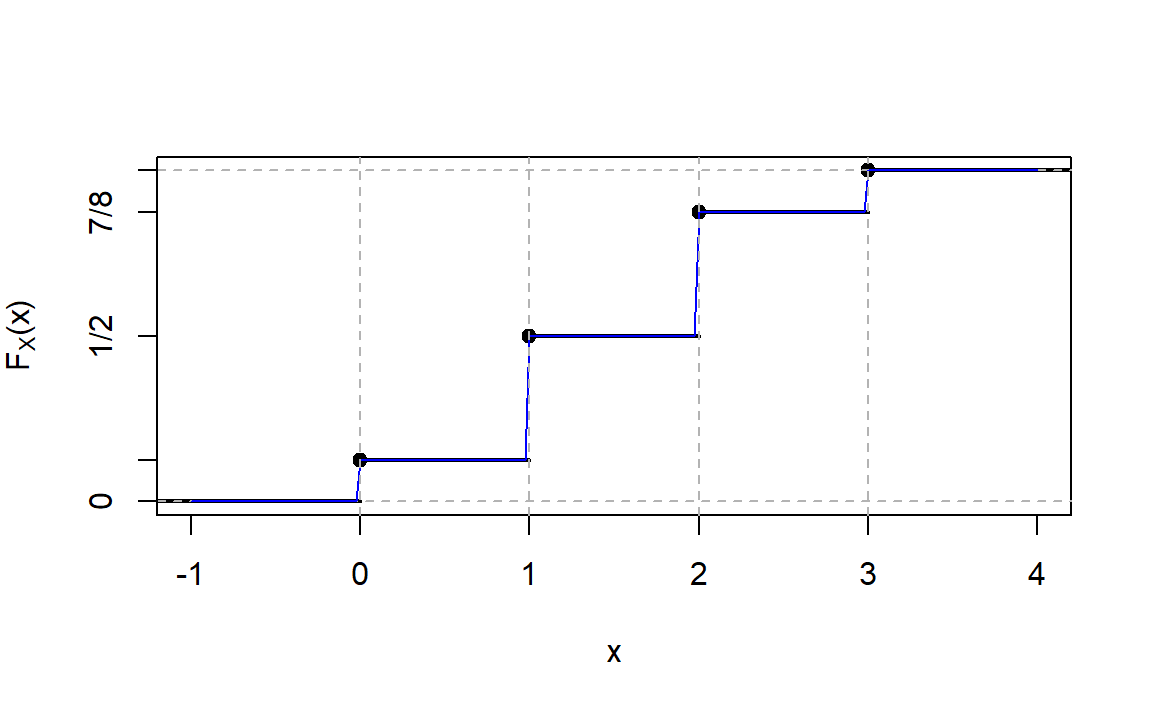
\includegraphics[width=0.7\linewidth]{Statistique_infentielle_files/figure-latex/unnamed-chunk-9-1} \end{center}

\textbf{Exemple:} Soit \(A\) un événement quelconque. On appelle variable aléatoire \emph{indicatrice} de cet événement \(A\), la variable aléatoire définie par: \[X(\omega) = \left\{ 
\begin{array}{l l}
 1 & \quad \text{si $\omega \in A$}\\
 0 & \quad \text{si $\omega \in \bar{A}$}\\   
  \end{array} \right.\]

et notée \(X=1_A\). Ainsi: \[P(X=1)=P(A)=p\]
\[P(X=0)=P(\bar{A})=1-p\]

La fonction de répartition de \(X\) est donc donnée par:

\[F(x) = \left\{ 
\begin{array}{l l}
 0 & \quad \text{si $x<0$}\\
  1-p & \quad \text{si $0 \leq x < 1$}\\ 
   1 & \quad \text{si $x \geq 1$}\\
\end{array} \right.\]

On peut prendre par exemple le cas d'un tirage d'une boule dans une urne
contenant 2 boules blanches et 3 boules noires. Soit
\(A:\text{"obtenir une boule blanche"}\) et \(X\) la variable indicatrice
de \(A\). La loi de probabilité de \(X\) est alors

\begin{longtable}[]{@{}ccc@{}}
\toprule
\(k\) & 0 & 1\tabularnewline
\midrule
\endhead
\(P(X = k)\) & \(\frac{3}{5}\) & \(\frac{2}{5}\)\tabularnewline
\bottomrule
\end{longtable}

et sa fonction de répartition est:

\[F(x) = \left\{ 
\begin{array}{l l}
 0 & \quad \text{si $x<0$}\\
  3/5 & \quad \text{si $0 \leq x < 1$}\\ 
   1 & \quad \text{si $x \geq 1$}\\
\end{array} \right.\]

\hypertarget{moments-dune-variable-aleatoire-discrete}{%
\section{Moments d'une variable aléatoire discrète}\label{moments-dune-variable-aleatoire-discrete}}

\hypertarget{esperance-mathematique}{%
\subsection*{Espérance mathématique}\label{esperance-mathematique}}
\addcontentsline{toc}{subsection}{Espérance mathématique}

\BeginKnitrBlock{definition}
\protect\hypertarget{def:unnamed-chunk-10}{}{\label{def:unnamed-chunk-10} }Pour une variable aléatoire discrète \(X\) de loi de probabilité \(p(.)\),
on définit l'\emph{espérance} de \(X\), notée \(E(X)\), par l'expression

\[E(X)=\sum_{i \in \mathbb{N}} x_{i} p(x_i)\]

En termes concrets, l'espérance de \(X\) est la moyenne pondérée des
valeurs que \(X\) peut prendre, les poids étant les probabilités que ces
valeurs soient prises.
\EndKnitrBlock{definition}

Reprenons l'exemple où on joue 3 fois à pile ou face. L'espérance
de \(X=\)``nombre de pile obtenus'' est égal à:
\[E(X)=0 \times \frac{1}{8}+1 \times \frac{3}{8}+2 \times \frac{3}{8}+3 \times \frac{1}{8}=1.5\]

Dans le cas de la loi uniforme sur \(X(\Omega)=\{x_{1},\ldots, x_{k}\}\),
c'est à dire avec équiprobabilité de toutes les valeurs \(p_{i}=1/k\), on
obtient: \[E(X)=\frac{1}{k} \sum_{i=1}^k x_{i}\] et dans ce cas \(E(X)\)
se confond avec la moyenne arithmétique simple \(\bar{x}\) des valeurs
possibles de \(X\).

Pour le jet d'un dé équilibré par exemple:
\[E(X)=\frac{1}{6} \sum_{i=1}^6 i=\frac{7}{2}=3.5\]

\hypertarget{esperance-dune-fonction-dune-variable-aleatoire}{%
\subsection*{Espérance d'une fonction d'une variable aléatoire}\label{esperance-dune-fonction-dune-variable-aleatoire}}
\addcontentsline{toc}{subsection}{Espérance d'une fonction d'une variable aléatoire}

\BeginKnitrBlock{theorem}[Théorème du transfert]
\protect\hypertarget{thm:unnamed-chunk-11}{}{\label{thm:unnamed-chunk-11} \iffalse (Théorème du transfert) \fi{} }Si X est une variable aléatoire discrète pouvant prendre ses valeurs
parmi les valeurs \(x_i\), \(i \geq 1\), avec des probabilités respectives
\(p(x_i)\), alors pour toute fonction réelle \(g\) on a

\[E(g(X)) = \sum_i g(x_i)p(x_i)\]
\EndKnitrBlock{theorem}

\BeginKnitrBlock{example}
\protect\hypertarget{exm:unnamed-chunk-12}{}{\label{exm:unnamed-chunk-12} }Soit \(X\) une variable aléatoire qui prend une des trois valeurs
\(\{-1,0,1\}\) avec les probabilités respectives

\[P(X=-1) = 0.2 \quad \quad P(X=0)=0.5 \quad \quad P(X=1) = 0.3\]

Calculer \(E(X^2)\).
\EndKnitrBlock{example}

\BeginKnitrBlock{solution}
\iffalse{} {Solution: } \fi{}\emph{Première approche}: Soit \(Y=X^2\). La distribution de \(Y\) est donnée par
\[\begin{aligned}
    P(Y=1) &= P(X=-1) + P(X=1) = 0.5 \\
    P(Y=0) &= P(X=0) = 0.5
  \end{aligned}\] Donc \[E(X^2)=E(Y) = 1(0.5) + 0(0.5) = 0.5\]

\emph{Deuxième approche}: En utilisant le théorème

\[\begin{aligned}
  E(X^2) &= (-1)^2(0.2) + 0^2(0.5) + 1^2 (0.3) \\
         &= 1(0.2+0.3)+0(0.5)=0.5
  \end{aligned}\]

Remarquer que \[0.5=E(X^2) \neq (E(X))^2 = 0.01\]
\EndKnitrBlock{solution}

\hypertarget{linearite-de-lesperance-proprietes-de-lesperance}{%
\subsubsection*{Linéarité de l'espérance Propriétés de l'espérance}\label{linearite-de-lesperance-proprietes-de-lesperance}}
\addcontentsline{toc}{subsubsection}{Linéarité de l'espérance Propriétés de l'espérance}

\begin{enumerate}
\def\labelenumi{\arabic{enumi}.}
\item
  \(E(X+a)=E(X)+a, \quad a \in \mathbb{R}\)\\
  résultat qui se déduit de:
  \[\sum_{i}p_{i}(x_{i}+a)= \sum_{i}p_{i}x_{i}+\sum_{i}ap_{i}=\sum_{i}p_{i}x_{i}+a \sum_{i}p_{i}=\sum_{i}p_{i}x_{i}+a\]
\item
  \(E(aX)=aE(X), \quad a\in \mathbb{R}\)\\
  il suffit d'écrire: \[\sum_{i}p_{i}a x_{i}=a\sum_{i}p_{i}x_{i}\]
\item
  \(E(X+Y)=E(X)+E(Y)\), \(X\) et \(Y\) étant deux variables aléatoire.
\end{enumerate}

On peut résumer ces trois propriétés en disant que l'espérance
mathématique est linéaire:
\[E(\lambda X + \mu Y)= \lambda E(X)+\mu E(Y), \quad \forall \lambda \in \mathbb{R}, \, \forall \mu \in \mathbb{R}.\]

\hypertarget{variance}{%
\subsection*{Variance}\label{variance}}
\addcontentsline{toc}{subsection}{Variance}

\BeginKnitrBlock{definition}
\protect\hypertarget{def:unnamed-chunk-14}{}{\label{def:unnamed-chunk-14} }La variance est un indicateur mesurant la dispersion des valeurs \(x_{i}\)
que peut prendre la v.a. \(X\) et son espérance \(E(X)\). On appelle
\textbf{variance} de X, que l'on note \(V(X)\), la quantité

\[V(X)=E\big[ (X-E(X))^2 \big]\] lorsque cette quantité existe.\\
C'est l'espérance mathématique du carré de la v.a. centrée \(X-E(X)\).
\EndKnitrBlock{definition}

On peut établir une autre formule pour le calcul de \(V(X)\):

\[V(X)=E(X^2)-E^2(X)\]

Or: \[\begin{aligned}
      V(X)&= E\left[X^2-2XE(X)+E^2(X)\right] \\
           &=E(X^2)-E[2XE(X)]+ E[E^2(X)]\\
           &=E(X^2)-2E^2(X)+E^2(X) \\ 
           &=E(X^2)-E^2(X)
    \end{aligned}\]

On cherche \(V(X)\) où \(X\) est le nombre obtenu lors du jet d'un dé
équilibré. On a vu dans l'exemple
que \(E(X) = \frac{7}{2}\). De plus,

\[\begin{aligned}
  E(X^2) &= 1^2 \bigg(\frac{1}{6}\bigg) + 2^2 \bigg(\frac{1}{6}\bigg) + 3^2 \bigg(\frac{1}{6}\bigg) + 4^2 \bigg(\frac{1}{6}\bigg) + 5^2 \bigg(\frac{1}{6}\bigg) + 6^2 \bigg(\frac{1}{6}\bigg) \\
        &=\bigg(\frac{1}{6}\bigg) (91) = \frac{91}{6}.\end{aligned}\] Et
donc

\[V(X) = \frac{91}{6} - \bigg(\frac{7}{2}\bigg)^2 = \frac{35}{12}\]

\textbf{Propriétés de la variance}

\begin{enumerate}
\def\labelenumi{\arabic{enumi}.}
\item
  \(V(X) \geq 0\)
\item
  \(V(X+a)=V(X)\)\\
  en effet: \[\begin{aligned}
     V(X+a)   &= E\big[\left[X+a-E(X+a)\right]^2\big] \\ 
          &=E\big[\left[X+a-E(X)-a\right]^2\big] \\ 
          &=E\big[\left[X-E(X)\right]^2\big] \\
          &=V(X). 
     \end{aligned}\]
\item
  \(V(aX)=a^2V(X)\)\\
  en effet: \[\begin{aligned}
     V(aX)  &= E\big[\left[aX-E(aX)\right]^2\big] \\
        &=E\big[\left[aX-aE(X)\right]^2\big] \\ 
        &=E\big[a^2\left[X-E(X)\right]^2\big] \\
        &=a^2\big[E\left[X-E(X)\right]^2\big] \\
        &= a^2V(X). 
     \end{aligned}\]
\end{enumerate}

\hypertarget{ecart-type}{%
\subsection*{Ecart-type}\label{ecart-type}}
\addcontentsline{toc}{subsection}{Ecart-type}

\BeginKnitrBlock{definition}
\protect\hypertarget{def:unnamed-chunk-15}{}{\label{def:unnamed-chunk-15} }La racine carrée de \(V(X)\) est appelée l'\textbf{\emph{écart-type}} de \(X\), qui se
note \(\sigma_{X}\). On a

\[\sigma_{X} = \sqrt{V(X)}\]

\(\sigma_{X}\) s'exprime dans les mêmes unités de mesure que la variable
aléatoire \(X\).
\EndKnitrBlock{definition}

A noter:

\begin{itemize}
\item
  L'écart type sert à mesurer la dispersion d'un ensemble de données.
\item
  Plus il est faible, plus les valeurs sont regroupées autour de la
  moyenne.
\item
  Exemple: La répartition des notes d'une classe. Plus l'écart type
  est faible, plus la classe est homogène.
\item
  L'espérance et l'écart-type sont reliés par l'\emph{inégalité de
  Bienaymé-Tchebychev}.
\end{itemize}

\hypertarget{inegalite-de-bienayme-tchebychev}{%
\subsubsection*{Inégalité de Bienaymé-Tchebychev}\label{inegalite-de-bienayme-tchebychev}}
\addcontentsline{toc}{subsubsection}{Inégalité de Bienaymé-Tchebychev}

\BeginKnitrBlock{theorem}
\protect\hypertarget{thm:unnamed-chunk-16}{}{\label{thm:unnamed-chunk-16} }Soit \(X\) une variable aléatoire d'espérance \(\mu\) et de variance
\(\sigma^2\). Pour tout \(\varepsilon > 0\), on a l'inégalité suivante:
\[P\left(|X-E(X)| \geq \varepsilon \right) \leq \frac{\sigma^2}{\varepsilon^2}\]

On peut l'écrire autrement. Soit \(k=\varepsilon/\sigma\).
\[P\left(|X-E(X)| \geq k\sigma \right) \leq \frac{1}{k^2}\]
\EndKnitrBlock{theorem}

\begin{rmdinsight}
{Importance}: Cette inégalité relie la probabilité pour \(X\) de
s'écarter de sa moyenne \(E(X)\), à sa variance qui est justement un
indicateur de dispersion autour de la moyenne de la loi. Elle montre
quantitativement que ``plus l'écart type est faible, plus la probabilité
de s'écarter de la moyenne est faible''.
\end{rmdinsight}

\BeginKnitrBlock{theorem}[Inégalité de Markov]
\protect\hypertarget{thm:unnamed-chunk-18}{}{\label{thm:unnamed-chunk-18} \iffalse (Inégalité de Markov) \fi{} }Soit \(X\) une variable aléatoire à valeur non
négatives. Pour tout réel \(a > 0\) \[P(X>a) \leq \frac{E(X)}{a}\]
\EndKnitrBlock{theorem}

\hypertarget{moments-non-centres-et-centres}{%
\subsection*{Moments non centrés et centrés}\label{moments-non-centres-et-centres}}
\addcontentsline{toc}{subsection}{Moments non centrés et centrés}

On appelle moment non centré d'ordre \(r \in \mathbb{N^*}\) de \(X\) la
quantité, lorsqu'elle existe:
\[m_{r}(X)=\sum_{i \in \mathbb{N} } x_{i}^r p(x_{i})=E(X^r).\] Le moment
centré d'ordre \(r \in \mathbb{N^*}\) est la quantité, lorsqu'elle existe:
\[\mu_{r}(X)=\sum_{i \in \mathbb{N} } p_{i}\left[x_{i}-E(X)\right]^r=E\left[X-E(X)\right]^r.\]

Les premiers moments sont: \[m_{1}(X)=E(X), \quad \mu_{1}(X)=0\]
\[\mu_{2}(X)=V(X)=m_{2}(X)-m_{1}^2(X)\]

\hypertarget{couple-de-variables-aleatoires-discretes}{%
\section{Couple de variables aléatoires discrètes}\label{couple-de-variables-aleatoires-discretes}}

Considérons deux variables aléatoires discrètes \(X\) et \(Y\). Il nous faut
pour modéliser le problème une fonction qui nous donne la probabilité
que \((X = x_i )\) en même temps que \((Y = y_j )\). C'est la loi de
probabilité conjointe.

Soit \(X\) et \(Y\) deux variables aléatoires réelles discrètes, définies
sur un espace probabilisé \((\Omega,\mathcal{A},P)\) et que

\[\begin{aligned}
  X(\Omega) &= \{x_1,x_2,\ldots,x_l\} \\
  Y(\Omega) &= \{y_1,y_2,\ldots,y_k\} \\
            & \quad (l \text{ et } k \in \mathbb{N})\end{aligned}\]

La \textbf{\emph{loi du couple \((X,Y)\)}}, dite \textbf{loi de probabilité conjointe ou
simultanée}, est entièrement définie par les probabilités:

\[p_{ij} = P(X=x_i;Y=y_j) = P(\{X=x_i\}\cap\{Y=y_j\})\]

On a

\[p_{ij} \geq 0 \quad \text{et} \quad \sum_{i=1}^{l} \sum_{j=1}^{k} p_{ij} = 1\]

Le couple \((X,Y)\) s'appelle variable aléatoire à deux dimensions et peut
prendre \(l\times k\) valeurs.

\hypertarget{table-de-probabilite-conjointe}{%
\subsection*{Table de probabilité conjointe}\label{table-de-probabilite-conjointe}}
\addcontentsline{toc}{subsection}{Table de probabilité conjointe}

Les probabilités \(p_{ij}\) peuvent être présentées dans un tableau à deux
dimensions qu'on appelle table de probabilité conjointe:

\begin{longtable}[]{@{}ccccccc@{}}
\caption{Table de probabilité conjointe}\tabularnewline
\toprule
\(X\)\textbackslash{}\(Y\) & \(y_1\) & \(y_2\) & \(\ldots\) & \(y_j\) & \(\ldots\) & \(y_k\)\tabularnewline
\midrule
\endfirsthead
\toprule
\(X\)\textbackslash{}\(Y\) & \(y_1\) & \(y_2\) & \(\ldots\) & \(y_j\) & \(\ldots\) & \(y_k\)\tabularnewline
\midrule
\endhead
\(x_1\) & \(p_{11}\) & \(p_{12}\) & & \(p_{1j}\) & & \(p_{1k}\)\tabularnewline
\(x_2\) & \(p_{21}\) & \(p_{22}\) & & \(p_{2j}\) & & \(p_{2k}\)\tabularnewline
\(\vdots\) & & & & & &\tabularnewline
\(x_i\) & \(p_{i1}\) & \(p_{i2}\) & & \(p_{ij}\) & & \(p_{ik}\)\tabularnewline
\(\vdots\) & & & & & &\tabularnewline
\(x_l\) & \(p_{l1}\) & \(p_{l2}\) & & \(p_{lj}\) & & \(p_{lk}\)\tabularnewline
\bottomrule
\end{longtable}

A la première ligne figure l'ensemble des valeurs de \(Y\) et à la
première colonne figure l'ensemble des valeurs de \(X\). La probabilité
\(p_{ij} = P(X=x_i;Y=y_j)\) est à l'intersection de la \(i^{e}\) et de la
\(j^{e}\) colonne.

\hypertarget{lois-marginales}{%
\subsection*{Lois marginales}\label{lois-marginales}}
\addcontentsline{toc}{subsection}{Lois marginales}

Lorsqu'on connaît la loi conjointe des variables aléatoires \(X\) et \(Y\),
on peut aussi s'intéresser à la loi de probabilité de \(X\) seule et de
\(Y\) seule. Ce sont les lois de probabilité marginales.

\begin{itemize}
\item
  Loi marginale de \(X\):
  \[p_{i.} = P(X=x_i) = P[\{X=x_i\}\cap \Omega] = \sum_{j=1}^k p_{ij} \quad \quad \forall \, i=1,2,\ldots,l\]
\item
  Loi marginale de \(Y\):
  \[p_{.j} = P(Y=y_j) = P[ \Omega \cap \{Y=y_j\}] = \sum_{i=1}^l p_{ij} \quad \quad \forall \, j=1,2,\ldots,k\]
\end{itemize}

On peut calculer les lois marginales directement depuis la table de la
loi conjointe. La loi marginale de \(X\) est
calculée en faisant les totaux par ligne, tandis que celle de \(Y\) l'est
en faisant les totaux par colonne.

C'est le fait que les lois de \(X\) et \(Y\) individuellement puissent être
lues dans les marges du tableau qui leur vaut leur nom de lois
marginales.

\begin{longtable}[]{@{}cccccccc@{}}
\caption{Table de probabilité conjointe avec les lois marginales}\tabularnewline
\toprule
\(X\)\textbackslash{}\(Y\) & \(y_1\) & \(y_2\) & \(\ldots\) & \(y_j\) & \(\ldots\) & \(y_k\) & Marginale de \(X\)\tabularnewline
\midrule
\endfirsthead
\toprule
\(X\)\textbackslash{}\(Y\) & \(y_1\) & \(y_2\) & \(\ldots\) & \(y_j\) & \(\ldots\) & \(y_k\) & Marginale de \(X\)\tabularnewline
\midrule
\endhead
\(x_1\) & \(p_{11}\) & \(p_{12}\) & & \(p_{1j}\) & & \(p_{1k}\) & \(p_{1.}\)\tabularnewline
\(x_2\) & \(p_{21}\) & \(p_{22}\) & & \(p_{2j}\) & & \(p_{2k}\) & \(p_{2.}\)\tabularnewline
\(\vdots\) & & & & & & &\tabularnewline
\(x_i\) & \(p_{i1}\) & \(p_{i2}\) & & \(p_{ij}\) & & \(p_{ik}\) & \(p_{i.}\)\tabularnewline
\(\vdots\) & & & & & & &\tabularnewline
\(x_l\) & \(p_{l1}\) & \(p_{l2}\) & & \(p_{lj}\) & & \(p_{lk}\) & \(p_{l.}\)\tabularnewline
Marginale de \(Y\) & \(p_{.1}\) & \(p_{.2}\) & & \(p_{.l}\) & & \(p_{.k}\) & 1\tabularnewline
\bottomrule
\end{longtable}

\begin{rmdexercise}
On tire au hasard 3 boules d'une urne contenant 3 boules rouges, 4
blanches et 5 noires. \(X\) et \(Y\) désignent respectivement le nombre
de boules rouges et celui de boules blanches tirées. Déterminer la loi
de probabilité conjointe du couple \((X,Y)\) ainsi que les lois
marginales de \(X\) et de \(Y\).
\end{rmdexercise}

\hypertarget{lois-conditionnelles}{%
\subsection*{Lois conditionnelles}\label{lois-conditionnelles}}
\addcontentsline{toc}{subsection}{Lois conditionnelles}

Pour chaque valeur \(y_j\) de \(Y\) telle que \(p_{.j} = P(Y=y_j) \neq 0\) on
peut définir la loi conditionnelle de \(X\) sachant \(Y=y_j\) par

\[p_{i/j} = P(X=x_i / Y=y_j) = \frac{P(X=x_i;Y=y_j)}{P(Y=y_j)} = \frac{p_{ij}}{p_{.j}} \quad \quad \forall i = 1,2,\ldots,l\]

De même on définit la loi de \(Y\) sachant \(X=x_i\) par

\[p_{j/i} = P(Y=y_j / X=x_i) = \frac{P(X=x_i;Y=y_j)}{P(X=x_i)} = \frac{p_{ij}}{p_{i.}} \quad \quad \forall j = 1,2,\ldots,k\]

\hypertarget{independance-de-variables-aleatoires}{%
\subsection*{Indépendance de variables aléatoires}\label{independance-de-variables-aleatoires}}
\addcontentsline{toc}{subsection}{Indépendance de variables aléatoires}

\BeginKnitrBlock{theorem}
\protect\hypertarget{thm:unnamed-chunk-20}{}{\label{thm:unnamed-chunk-20} }On dit que deux v.a.r.d sont indépendantes si et seulement si

\[P(X=x_i;Y=y_j) = P(X=x_i) P(Y=y_j) \quad \quad \forall \, i = 1,2,\ldots,l \text{ et }  j = 1,2,\ldots,k\]
\EndKnitrBlock{theorem}

On montre que

\[P(\{X\in A\} \cap \{Y \in B\}) = P(\{X\in A\}) P(\{Y \in B\}) \quad \quad \forall \,\, A \text{ et } B \in \mathcal{A}\]

\textbf{Propriétés}

Soit deux v.a.r.d. \(X\) et \(Y\),

\begin{enumerate}
\def\labelenumi{\arabic{enumi}.}
\item
  \(E(X+Y)=E(X)+E(Y)\)
\item
  Si \(X\) et \(Y\) sont indépendantes alors \(E(XY)=E(X)E(Y)\). Mais la
  réciproque n'est pas toujours vraie.
\end{enumerate}

\hypertarget{covariance}{%
\subsection*{Covariance}\label{covariance}}
\addcontentsline{toc}{subsection}{Covariance}

Soit \(X\) et \(Y\) deux v.a.r.d. On appelle \textbf{\emph{covariance}} de \(X\) et de
\(Y\) la valeur si elle existe de

\[Cov(X,Y) = E[(X-E(X))(Y-E(Y))] = \sum_i \sum_j (x_i-E(X))(y_j-E(Y)) p_{ij}\]

qu'on peut calculer en utilisant la formule suivante

\[Cov(X,Y) = E(XY) - E(X)E(Y)\]

\textbf{Propriétés}

\begin{itemize}
\item
  \(Cov(X,Y)=Cov(Y,X)\)
\item
  \(Cov(aX_1+bX_2,Y) = a Cov(X_1,Y) + b Cov(X_2,Y)\)
\item
  \(V(X+Y)= V(X) + V(Y) + 2 Cov(X,Y)\)
\item
  Si \(X\) et \(Y\) sont indépendantes alors

  \begin{itemize}
  \item
    \(Cov(X,Y) = 0\) (la réciproque n'est pas vraie)
  \item
    \(V(X+Y) = V(X) + V(Y)\) (la réciproque n'est pas vraie)
  \end{itemize}
\end{itemize}

\hypertarget{coefficient-de-correlation-lineaire}{%
\subsection*{Coefficient de corrélation linéaire}\label{coefficient-de-correlation-lineaire}}
\addcontentsline{toc}{subsection}{Coefficient de corrélation linéaire}

On appelle coefficient de corrélation linéaire de \(X\) et de \(Y\) la
valeur définie par

\[\rho = \rho(X,Y) = \frac{Cov(X,Y)}{\sqrt{V(X)V(Y)}} = \frac{Cov(X,Y)}{\sigma_X \sigma_Y}\]

On peut montrer que \[-1 \leq \rho(X,Y) \leq 1\]

Pour le montrer on peut partir du fait que la variance est toujours
positive ou nulle. Donc
\(V(\frac{X}{\sigma_X} + \frac{Y}{\sigma_Y}) \geq 0\) et
\(V(\frac{X}{\sigma_X} - \frac{Y}{\sigma_Y}) \geq 0\).

\textbf{Interprétation de \(\rho\)}

\begin{itemize}
\item
  Le coefficient de corrélation est une mesure du degré de linéarité
  entre \(X\) et \(Y\).
\item
  Les valeurs de \(\rho\) proches de \(1\) ou \(-1\) indiquent une linéarité
  quasiment rigoureuse entre \(X\) et \(Y\).
\item
  Les valeurs de \(\rho\) proche de 0 indiquent une absence de toute
  relation linéaire.
\item
  Lorsque \(\rho(X,Y)\) est positif, \(Y\) a tendance à augmenter si \(X\)
  en fait autant.
\item
  Lorsque \(\rho(X,Y) < 0\), \(Y\) a tendance à diminuer si \(X\) augmente.
\item
  Si \(\rho(X,Y) =0\), on dit que ces deux statistiques sont non
  corrélées.
\end{itemize}

\hypertarget{lois-usuelles-discretes}{%
\section{Lois usuelles discrètes}\label{lois-usuelles-discretes}}

\hypertarget{loi-uniforme-discrete-mathcalun}{%
\subsection{\texorpdfstring{Loi uniforme discrète \(\mathcal{U}(n)\)}{Loi uniforme discrète \textbackslash mathcal\{U\}(n)}}\label{loi-uniforme-discrete-mathcalun}}

\BeginKnitrBlock{definition}
\protect\hypertarget{def:unnamed-chunk-21}{}{\label{def:unnamed-chunk-21} }Une distribution de probabilité suit une loi uniforme lorsque toutes les
valeurs prises par la variable aléatoire sont équiprobables. Si \(n\) est
le nombre de valeurs différentes prises par la variable aléatoire alors
on a:

\[\label{eq:unif}
    P(X=x_i)=\frac{1}{n} \qquad \forall \, i \in \{1,\ldots, n\}\]
\EndKnitrBlock{definition}

\textbf{Exemple:} La distribution des chiffres obtenus au lancer de dé (si ce dernier est
non pipé) suit une loi uniforme dont la loi de probabilité est la
suivante :

\begin{longtable}[]{@{}ccccccc@{}}
\toprule
\(x_i\) & 1 & 2 & 3 & 4 & 5 & 6\tabularnewline
\midrule
\endhead
\(P(X = x_i)\) & \(\frac{1}{6}\) & \(\frac{1}{6}\) & \(\frac{1}{6}\) & \(\frac{1}{6}\) & \(\frac{1}{6}\) & \(\frac{1}{6}\)\tabularnewline
\bottomrule
\end{longtable}

\textbf{Moments de loi uniforme discrète}

Dans le \textbf{cas particulier} d'une loi uniforme discrète où chaque valeur
de la variable aléatoire \(X\) correspond à son rang, i.e.
\(x_i=i \, \, \forall i \in \{1,\ldots, n\}\), on a:
\[E(X)=\frac{n+1}{2} \quad \text{et} \quad V(X)=\frac{n^2-1}{12}\] La
démonstration de ces résultats est établie en utilisant les égalités
(cf.~Annexe)
\[\sum_{i=1}^n i=\frac{n(n+1)}{2} \quad \text{et} \quad \sum_{i=1}^n i^2=\frac{n(n+1)(2n+1)}{6}.\]

En revenant à l'exemple du lancer du dé de cette section, on peut
calculer directement les moments de \(X\): \[E(X)=\frac{6+1}{2}=3.5\] et
\[V(X)=\frac{6^2-1}{12}=\frac{35}{12}\simeq 2.92.\]

\hypertarget{loi-de-bernoulli-mathcalbp}{%
\subsection{\texorpdfstring{Loi de Bernoulli \(\mathcal{B}(p)\)}{Loi de Bernoulli \textbackslash mathcal\{B\}(p)}}\label{loi-de-bernoulli-mathcalbp}}

\BeginKnitrBlock{definition}
\protect\hypertarget{def:unnamed-chunk-22}{}{\label{def:unnamed-chunk-22} }On réalise une expérience dont le résultat sera interprété soit comme un
succès soit comme un échec. On définit alors la variable aléatoire \(X\)
en lui donnant la valeur 1 lors d'un succès et 0 lors d'un échec
(variable indicatrice). La loi de probabilité de \(X\) est alors

\begin{align}
    &p(1)=P(X=1)=p \label{eq:bern} \\ 
    &p(0)=P(X=0)= 1-p=q \notag
\end{align}

où \(p\) est la probabilité d'un succès, \(0 \leq p \leq 1\).

Une variable aléatoire \(X\) est dite de \textbf{Bernoulli}
\(X \sim \mathcal{B} \left({p}\right)\) s'il existe un nombre
\(p \, \in \, ]0,1[\) tel que la loi de probabilité de \(X\) soit donnée par \eqref{eq:bern}.
\EndKnitrBlock{definition}

La fonction de répartition est définie par: \[F(x) = 
       \left\{
       \begin{array}{ll}
         0 & \quad \text{si $x < 0$} \\
         1 - p & \quad \text{si $0 \leq x < 1$} \\
         1 & \quad \text{si $x \geq 1$}.
       \end{array}
       \right.\]

L'espérance la loi de Bernoulli est \(p\), en effet

\[E(X) =1 \times P(X=1)+0 \times P(X=0)=P(X=1)=p\]

La variance la loi de Bernoulli est \(np\), en effet

\[V(X) =E(X^2)-E^2(X)=p-p^2=p(1-p)=pq\] car
\[E(X^2) =1^2\times P(X=1)+0^2 \times P(X=0)=P(X=1)=p\]

\hypertarget{loi-binomiale-mathcalbnp}{%
\subsection{\texorpdfstring{Loi Binomiale \(\mathcal{B}(n,p)\)}{Loi Binomiale \textbackslash mathcal\{B\}(n,p)}}\label{loi-binomiale-mathcalbnp}}

\BeginKnitrBlock{rmdtip}
Décrite pour la première fois par \emph{Isaac Newton} en 1676 et démontrée pour la première fois par le mathématicien suisse \emph{Jacob Bernoulli} en 1713, la loi binomiale est l'une des distributions de probabilité les plus fréquemment rencontrées en statistique appliquée.
\EndKnitrBlock{rmdtip}

Supposons qu'on exécute maintenant \(n\) épreuves \textbf{indépendantes},
chacune ayant \(p\) pour probabilité de succès et \(1-p\) pour probabilité
d'échec. La variable aléatoire \(X\) qui compte \textbf{le nombre de succès}
sur l'ensemble des \(n\) épreuves est dite variable aléatoire
\textbf{binomiale} de paramètres \(n\) et \(p\).

\BeginKnitrBlock{rmdinsight}
Une variable de Bernoulli n'est donc qu'une variable binomiale de paramètres \((1,p)\).
\EndKnitrBlock{rmdinsight}

\BeginKnitrBlock{definition}
\protect\hypertarget{def:unnamed-chunk-25}{}{\label{def:unnamed-chunk-25} }Si on effectue \(n\) épreuves successives indépendantes où on note à
chaque fois la réalisation ou non d'un certain événement \(A\), on obtient une suite de la forme \(AA\bar{A}A\bar{A}\ldots \bar{A}AA\). Soit \(X\) le nombre de réalisations de \(A\). On définit ainsi une v.a. \(X\) qui suit une loi binomiale de paramètres \(n\) et \(p=P(A)\), caractérisée par
\(X(\Omega)=\{0, 1,\ldots, n\}\) :

\begin{equation}
    P(X=k)=\binom{n}{k}p^k (1-p)^{n-k} \qquad 0\leq k \leq n
    \label{eq:binom}
\end{equation}

On écrit \(X \sim \mathcal{B} \left({n, p}\right)\). Donc la loi binomiale modélise le nombre de réalisations de \(A\) (succès) obtenues lors de la répétition indépendante et identique de \(n\) épreuves de Bernoulli.
\EndKnitrBlock{definition}

\BeginKnitrBlock{rmdinsight}
Pour établir \eqref{eq:binom} il faut remarquer que \(\binom{n}{k}\) est le nombre d'échantillons de taille \(n\) comportant exactement \(k\) événements \(A\), de probabilité \(p^k\), indépendamment de l'ordre, et donc \(n-k\) événements \(\bar{A}\), de probabilité \((1-p)^{n-k}\).
\EndKnitrBlock{rmdinsight}

\textbf{Remarque:} Il est possible d'obtenir aisément les valeurs des combinaisons de la loi binomiale en utilisant le triangle de Pascal.

En utilisant la formule du binôme de Newton, on vérifie
bien que c'est une loi de probabilité:

\[{\sum_{k=0}^nP(X=k)=\sum_{k=0}^n\binom{n}{k} p^{k}(1-p)^{n-k}=[p+(1-p)]^n=1}\]

\textbf{Exemple:} On jette cinq pièces équilibrées. Les résultats sont supposés
indépendants. Donner la loi de probabilité de la variable \(X\) qui compte
le nombre de piles obtenus.

\textbf{Moments de la loi Binomiale}

Pour calculer facilement les moments de cette loi, nous allons associer
à chaque épreuve \(i\), \(1\leq i \leq n\), une v.a. de Bernoulli (variable
indicatrice sur \(A\)): \[{1}_A=X_i = \left\{ 
\begin{array}{l l}
 1 & \quad \text{si $A$ est réalisé}\\
 0 & \quad \text{si $\bar{A}$ est réalisé}\\ 
  \end{array} \right.\] On peut écrire alors:
\(X=\sum_{i=1}^nX_i=X_1+X_2+\ldots+X_n\), ce qui nous permet de déduire
aisément: \[\begin{aligned}
    E(X)&=E\left(\sum_{i=1}^nX_i\right)=\sum_{i=1}^nE(X_i)=np \\
    \text{et} \nonumber \\
    V(X)&=V\left(\sum_{i=1}^nX_i\right)=\sum_{i=1}^nV(X_i)=np(1-p) \quad \text{car les v.a. $X_i$ sont indépendantes.}
  \end{aligned}\]

Le calcul direct des moments de \(X\) peut s'effectuer à partir de la
définition générale, mais de façon beaucoup plus laborieuse:
\[\begin{aligned}
 E(X)&= \sum_{k=0}^nk \binom{n}{k} p^{k}(1-p)^{n-k}=\sum_{k=1}^nk \frac{n!}{k!(n-k)!} p^{k}(1-p)^{n-k} \\
 &= \sum_{k=1}^n\frac{n!}{(k-1)!(n-k)!} p^{k}(1-p)^{n-k}= np \sum_{k=1}^n\frac{(n-1)!}{(k-1)!(n-k)!} p^{k-1}(1-p)^{n-k} \\ 
 &= np \sum_{j=0}^{n-1}\frac{(n-1)!}{j!(n-1-j)!}p^j (1-p)^{n-1-j} =np \sum_{j=0}^{n-1}\binom{n-1}{j} p^{j}(1-p)^{n-1-j} \\
 &= np [p+(1-p)]^{n-1}=np
 \end{aligned}\]

Pour obtenir \(E(X^2)\) par un procédé de calcul identique, on passe par
l'intermédiaire du moment factoriel \(E[X(X-1)]=E(X^2)-E(X)\):
\[\begin{aligned}
  E[X(X-1)]&= \sum_{k=0}^nk(k-1) \frac{n!}{k!(n-k)!} p^{k}(1-p)^{n-k} \\ 
  &= n(n-1)p^2 \sum_{k=2}^{n}\frac{(n-2)!}{(k-2)!(n-k)!} p^{k-2}(1-p)^{n-k} \\ &= n(n-1)p^2 \sum_{j=0}^{n-2}\binom{n-2}{j} p^{j}(1-p)^{n-2-j} \\
  &= n(n-1)p^2[p+(1-p)]^{n-2}= n(n-1)p^2
   \end{aligned}\] On en déduit alors:
\[E(X^2)=E[X(X-1)]+E(X)= n(n-1)p^2+np,\] puis: \[\begin{aligned}
   V(X)&=n(n-1)p^2+np-(np)^2 \\ &=n^2p^2+np(1-p)-n^2p^2 \\ &=np(1-p).
  \end{aligned}\]

Le nombre de résultats pile apparus au cours de \(n\) jets d'une pièce de
monnaie suit une loi binomiale \(\mathcal{B} \left({n, 1/2}\right)\):
\[P(X=k)=\binom{n}{k}\left(\frac{1}{2}\right)^k \left(\frac{1}{2}\right)^{n-k}=\frac{\binom{n}{k}}{2^n}, \quad 0\leq k \leq n\]
avec \(E(X)=n/2\) et \(V(X)=n/4\).

Le nombre \(N\) de boules rouges apparues au cours de \(n\) tirages avec
remise dans une urne contenant deux rouges, trois vertes et une noire
suit une loi binomiale \(\mathcal{B} \left({n, 1/3}\right)\):
\[P(N=k)=\binom{n}{k}\left(\frac{1}{3}\right)^k \left(\frac{2}{3}\right)^{n-k}=\binom{n}{k} \frac{2^{n-k}}{3^n}, \quad 0\leq k \leq n\]
avec \(E(X)=n/3\) et \(V(X)=2n/9\).

\BeginKnitrBlock{theorem}
\protect\hypertarget{thm:unnamed-chunk-27}{}{\label{thm:unnamed-chunk-27} }Si \(X_1 \sim \mathcal{B} \left({n_1, p}\right)\) et
\(X_2 \sim \mathcal{B} \left({n_2, p}\right)\), les v.a. \(X_1\) et \(X_2\)
étant indépendantes, alors
\(X_1+X_2 \sim \mathcal{B} \left({n_1+n_2, p}\right)\). Ceci résulte de la
définition d'une loi binomiale puisqu'on totalise ici le résultat de
\(n_1+n_2\) épreuves indépendantes.
\EndKnitrBlock{theorem}

\hypertarget{loi-de-poisson-mathcalplambda}{%
\subsection*{\texorpdfstring{Loi de Poisson \(\mathcal{P}(\lambda)\)}{Loi de Poisson \textbackslash mathcal\{P\}(\textbackslash lambda)}}\label{loi-de-poisson-mathcalplambda}}
\addcontentsline{toc}{subsection}{Loi de Poisson \(\mathcal{P}(\lambda)\)}

\BeginKnitrBlock{rmdtip}
La loi de Poisson est découverte au début du XIX\(^e\) siècle par le
magistrat français \emph{Siméon-Denis Poisson}. Les variables aléatoires
de Poisson ont un champ d'application fort vaste, en particulier du
fait qu'on peut les utiliser pour approximer des variables
aléatoires binomiales de paramètres \((n,p)\) pour autant que \(n\) soit
grand et \(p\) assez petit pour que \(np\) soit d'ordre de grandeur
moyen.
\EndKnitrBlock{rmdtip}

\BeginKnitrBlock{definition}
\protect\hypertarget{def:unnamed-chunk-29}{}{\label{def:unnamed-chunk-29} }Une v.a. \(X\) suit une loi de Poisson de paramètre \(\lambda>0\) si c'est
une variable à valeurs entières, \(X(\Omega)=\mathbb{N}\), donc avec une
infinité de valeurs possibles, de probabilité: \[\label{eq:poisson}
    P(X=k)=e^{-\lambda} \frac{\lambda^k}{k!}, \quad k \in \mathbb{N}\]
Cette loi ne dépend qu'un seul paramètre réel positif \(\lambda\), avec
l'écriture symbolique \(X \sim \mathcal{P}(\lambda)\).
\EndKnitrBlock{definition}

Le développement en série entière de l'exponentielle
\(e^\lambda=\sum_{k=0}^{+\infty} \frac{\lambda^k}{k!}\) permet de
vérifier qu'il s'agit bien d'une loi de probabilité:
\[\sum_{k=0}^{\infty} P(X=k)=\sum_{k=0}^{\infty} e^{-\lambda} \frac{\lambda^k}{k!}=e^{-\lambda}\sum_{k=0}^{\infty} \frac{\lambda^k}{k!}=e^{-\lambda}e^{\lambda}=1\]

\textbf{Moments de loi de Poisson}

Le calcul de l'espérance mathématique se déduit du développement en
série entière de l'exponentielle: \[\begin{aligned}
    E(X)&=\sum_{k=0}^{\infty} k P(X=k)=\sum_{k=1}^{\infty} k e^{-\lambda} \frac{\lambda^k}{k!} \\
        &=e^{-\lambda} \sum_{k=1}^{\infty}  \frac{\lambda^k}{(k-1)!}=\lambda e^{-\lambda} \sum_{k=1}^{\infty}  \frac{\lambda^{k-1}}{(k-1)!} \\
        &= \lambda e^{-\lambda} \sum_{j=0}^{\infty}  \frac{\lambda^{j}}{j!}= \lambda e^{-\lambda}  e^{\lambda} \\
        &= \lambda.\end{aligned}\] Pour calculer la variance nous
n'allons pas calculer \(E(X^2)\) mais le moment factoriel \(E[X(X-1)]\) qui
s'obtient plus facilement, selon la méthode précédente:
\[\begin{aligned}
    E[X(X-1)] &=\sum_{k=0}^{\infty} k(k-1)P(X=k)=\sum_{k=2}^{\infty} k(k-1)  \,e^{-\lambda} \frac{\lambda^k}{k!} \\
        &=e^{-\lambda} \sum_{k=2}^{\infty}  \frac{\lambda^k}{(k-2)!}=\lambda^2 e^{-\lambda} \sum_{k=2}^{\infty}  \frac{\lambda^{k-2}}{(k-2)!} \\ 
        &= \lambda^2 e^{-\lambda} \sum_{j=0}^{\infty}  \frac{\lambda^{j}}{j!}= \lambda^2 e^{-\lambda}  e^{\lambda} = \lambda^2.\end{aligned}\]
On en déduit: \[\begin{aligned}
    V(X)&=E(X^2)-E^2(X)=E[X(X-1)]+E(X)-E^2(X) \\
        &=\lambda^2+\lambda-\lambda^2=\lambda.\end{aligned}\]

\BeginKnitrBlock{theorem}
\protect\hypertarget{thm:unnamed-chunk-30}{}{\label{thm:unnamed-chunk-30} }Si \(X\) et \(Y\) sont deux variables \textbf{indépendantes} suivant des lois de
Poisson
\[X \sim \mathcal{P}(\lambda) \quad \text{et} \quad Y \sim \mathcal{P}(\mu)\]
alors leur somme suit aussi une loi de Poisson:
\[X+Y \sim \mathcal{P}(\lambda+\mu).\]
\EndKnitrBlock{theorem}

\textbf{Exemple:} Soit \(X\) la variable aléatoire associée au nombre de micro-ordinateurs
vendus chaque jour dans le magasin. On suppose que \(X\) suit une loi de
Poisson de paramètre \(\lambda=5\). On écrit alors
\(X \sim \mathcal{P}(5).\)\\
La probabilité associée à la vente de 5 micro-ordinateurs se détermine
par : \[P(X=5)=e^{-5} \frac{5^5}{5!}=e^{-5}\simeq 0.1755\] La
probabilité de vendre au moins 2 micro-ordinateurs est égal à:
\[\begin{aligned}
P(X \geq 2)&=1-\left(e^{-5} \frac{5^0}{0!}+e^{-5} \frac{5^1}{1!}\right)\simeq 0.9596\end{aligned}\]
Le nombre moyen de micro-ordinateurs vendus chaque jour dans le magasin
est égal à 5 puisque \(E(X)=\lambda=5\).

\hypertarget{approximation-dune-loi-binomiale}{%
\subsection*{Approximation d'une loi binomiale}\label{approximation-dune-loi-binomiale}}
\addcontentsline{toc}{subsection}{Approximation d'une loi binomiale}

Le théorème de Poisson nous montre que si \(n\) est suffisamment grand et
\(p\) assez petit, alors on peut approcher la distribution d'une loi
binomiale de paramètres \(n\) et \(p\) par celle d'une loi de Poisson de
paramètre \(\lambda=np\), en effet
\[\text{si} \; n \rightarrow \infty \; \text{et}\; p \rightarrow 0 \; \text{alors} \; X: \mathcal{B}(n, p) \rightarrow \mathcal{P}(\lambda).\]

Une bonne approximation est obtenue si \(n \geq 50\) et \(np \leq 5\).

Dans ce contexte, la loi de Poisson est souvent utilisée pour modéliser
le nombre de succès lorsqu'on répète un très grand nombre de fois une
expérience ayant une chance très faible de réussir par une loi de
Poisson (nombre de personnes dans la population française atteints d'une
maladie rare, par exemple).

On cherche la probabilité de trouver au moins un centenaire parmi 200
personnes dans une population où une personne sur cent est un
centenaire.

La probabilité \(p=1/100=0.01\) étant faible et \(n=200\) étant suffisamment
grand, on peut modéliser le nombre \(X\) de centenaires pris parmi 200
personnes par la loi de Poisson de paramètre
\(\lambda=200 \times 0.01=2\). Donc on a:
\[P(X\geq 1)=1-P(X=0)=1-e^{-2}\simeq 0.86\]

Soit une v.a. \(X\) telle que \(X \sim \mathcal{B}(100, 0.01)\), les valeurs
des probabilités pour \(k\) de 0 à 5 ainsi que leur approximation à
\(10^{-3}\) avec une loi de Poisson de paramètre \(\lambda= np =1\) sont
données dans le tableau ci-dessous :

\begin{longtable}[]{@{}ccccccc@{}}
\toprule
\(k\) & 0 & 1 & 2 & 3 & 4 & 5\tabularnewline
\midrule
\endhead
\(P(X = k)\) & 0.366 & 0.370 & 0.185 & 0.061 & 0.015 & 0.000\tabularnewline
Approximation & 0.368 & 0.368 & 0.184 & 0.061 & 0.015 & 0.003\tabularnewline
\bottomrule
\end{longtable}

Dans le cas de cet exemple où \(n =100\) et \(np =1\), l'approximation de la
loi binomiale par une loi de poisson donne des valeurs de probabilités
identiques à \(10^{-3}\) près.

\hypertarget{loi-geometrique-ou-de-pascal-mathcalgp}{%
\subsection*{\texorpdfstring{Loi Géométrique ou de Pascal \(\mathcal{G}(p)\)}{Loi Géométrique ou de Pascal \textbackslash mathcal\{G\}(p)}}\label{loi-geometrique-ou-de-pascal-mathcalgp}}
\addcontentsline{toc}{subsection}{Loi Géométrique ou de Pascal \(\mathcal{G}(p)\)}

On effectue des épreuves successives indépendantes jusqu'à la
réalisation d'un événement particulier \(A\) de probabilité \(p=P(A)\) et on
note \(X\) le nombre aléatoire d'épreuves effectuées. On définit ainsi une
v.a. à valeurs entières de loi géométrique, ou de Pascal. A chaque
épreuve est associé l'ensemble fondamental \(\Omega=\{A, \bar{A}\}\) et
l'événement \(\{X=k\}\) pour \(k\in \mathbb{N^*}\) est représenté par une
suite de \(k-1\) événements \(\bar{A}\), terminée par l'événement \(A\):
\[\underbrace{\bar{A}\bar{A}\ldots \bar{A}}_{k-1}A\] D'où:

\begin{equation}
    P(X=k)=(1-p)^{k-1}p \quad \forall \, k \in \mathbb{N^*}
    \label{eq:geom}
\end{equation}
Cette loi peut servir à modéliser des temps de vie, ou des temps
d'attente, lorsque le temps est mesuré de manière discrète (nombre de
jours par exemple).

En utilisant la série entière \[\label{eq:serie_entiere}
        \sum_{k=0}^\infty x^k = 1/(1-x) \quad \text{pour} \quad |x|<1\]
on vérifie bien que c'est une loi de probabilité:

\[\begin{aligned}
\sum_{k=1}^\infty P(X=k)&= \sum_{k=1}^\infty (1-p)^{k-1}p = p \sum_{j=0}^\infty (1-p)^{j} \\
&= p \frac{1}{1-(1-p)}=1\end{aligned}\]

\textbf{Moments de loi Géométrique}

En dérivant la série entière
\eqref{eq:geom} ci-dessus, on obtient
\(\sum_{k=1}^\infty k x^{k-1}=1/(1-x)^2\). Ceci permet d'obtenir
l'espérance:
\[E(X)=\sum_{k=1}^\infty kp(1-p)^{k-1}=\frac{p}{[1-(1-p)]^2}=\frac{1}{p}\]

\begin{itemize}
\tightlist
\item
  En d'autres termes, si des épreuves indépendantes ayant une
  probabilité \(p\) d'obtenir un succès sont réalisés jusqu'à ce que le
  premier succès se produise, le nombre espéré d'essais nécessaires
  est égal à \(1/p\). Par exemple, le nombre espéré de jets d'un dé
  équilibré qu'il faut pour obtenir la valeur 1 est 6.
\end{itemize}

Le calcul de la variance se fait à partir du moment factoriel et en
utilisant la dérivée seconde de la série entière
\eqref{eq:geom}:
\(\sum_{k=2}^\infty k(k-1) x^{k-2} = 2/(1-x)^3\), Donc

\[\begin{aligned}
E[X(X-1)]&=\sum_{k=2}^\infty k(k-1)p(1-p)^{k-1} \\ &= p(1-p)\sum_{k=2}^\infty k(k-1)(1-p)^{k-2} \\
&=  \frac{2p(1-p)}{[1-(1-p)]^3}=\frac{2(1-p)}{p^2}\end{aligned}\] d'où
on déduit: \[V(X)=E[X(X-1)]+E(X)-E^2(X)=\frac{1-p}{p^2}.\]

Si l'on considère la variable aléatoire \(X\) ``nombre de naissances
observées jusqu'à l'obtention d'une fille'' avec p = 1/2 (même
probabilité de naissance d'une fille ou d'un garçon), alors X suit une
loi géométrique et on a pour tout \(k\in \mathbb{N^*}\):
\[P(X=k)=(1-1/2)^{k-1}(1/2)=1/2^k\] avec \(E(X)=2\) et \(V(X)=2.\)

\hypertarget{variables-aleatoires-continues}{%
\chapter*{Variables Aléatoires Continues}\label{variables-aleatoires-continues}}
\addcontentsline{toc}{chapter}{Variables Aléatoires Continues}

\hypertarget{densite-dune-variable-aleatoire-continue}{%
\section{Densité d'une variable aléatoire continue}\label{densite-dune-variable-aleatoire-continue}}

Dans les chapitres précédents nous avons traité des variables aléatoires
discrètes, c'est-à-dire de variables dont l'univers est fini ou infini
dénombrable. Il existe cependant des variables dont l'univers est infini
non dénombrable. On peut citer par exemple, l'heure d'arrivée d'un train
à une gare donnée ou encore la durée de vie d'un transistor. Désignons
par \(X\) une telle variable.

\BeginKnitrBlock{definition}
\protect\hypertarget{def:unnamed-chunk-32}{}{\label{def:unnamed-chunk-32} }\(X\) est une \textbf{variable aléatoire continue} s'il existe une fonction \(f\)
non négative définie pour tout \(x \in \mathbb{R}\) et vérifiant pour tout
ensemble \(B\) de nombres réels la propriété

\begin{equation}
P(X \in B) = \int_B f(x)dx
\label{eq:def}
\end{equation}

La fonction \(f\) est appelée \textbf{densité
de probabilité} de la variable aléatoire \(X\).
\EndKnitrBlock{definition}

Tous les problèmes de probabilité relatifs à \(X\) peuvent être traités
grâce à \(f\). Par exemple pour \(B=[a,b]\), on obtient grâce à l'équation
\eqref{eq:def}

\begin{equation}
P(a\le X \le b) = \int_a^bf(x)dx
\label{eq:probab}
\end{equation}

Graphiquement, \(P(a\le X \le b)\) est l'aire de la surface entre l'axe de
\(x\), la courbe correspondante à \(f(x)\) et les droites \(x=a\) et \(x=b\).
Voire Figure \ref{fig:paxb} et Figure \ref{fig:p2}.

\begin{figure}

{\centering 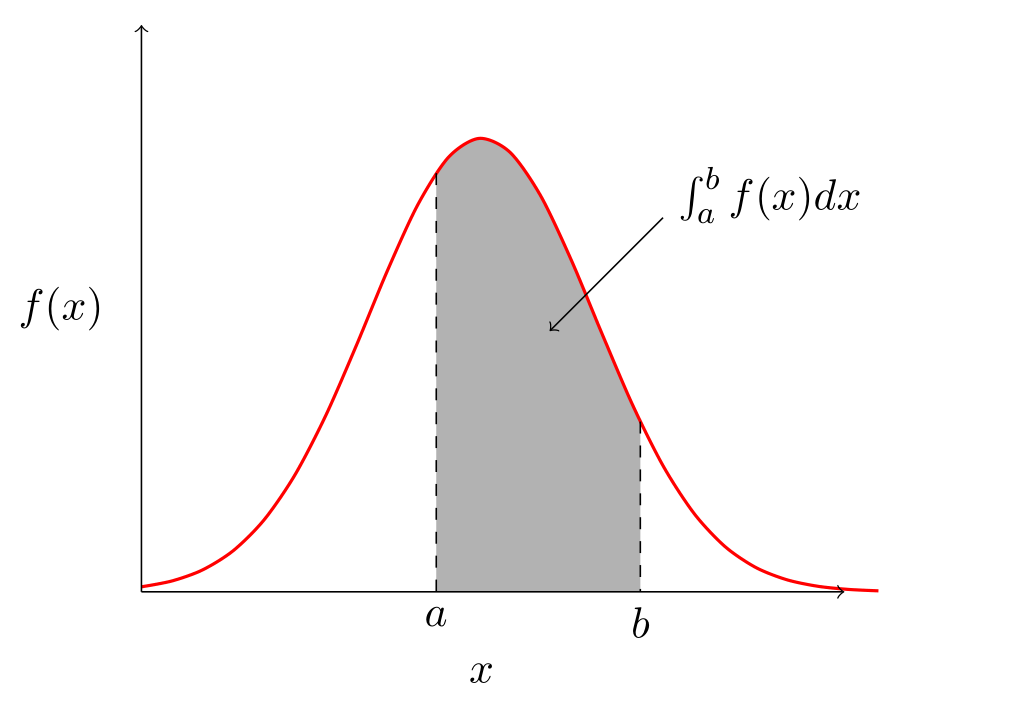
\includegraphics[width=0.7\linewidth]{img/paxb} 

}

\caption{$P(a \leq X \leq B)=$ surface grisée}\label{fig:paxb}
\end{figure}

\begin{figure}

{\centering 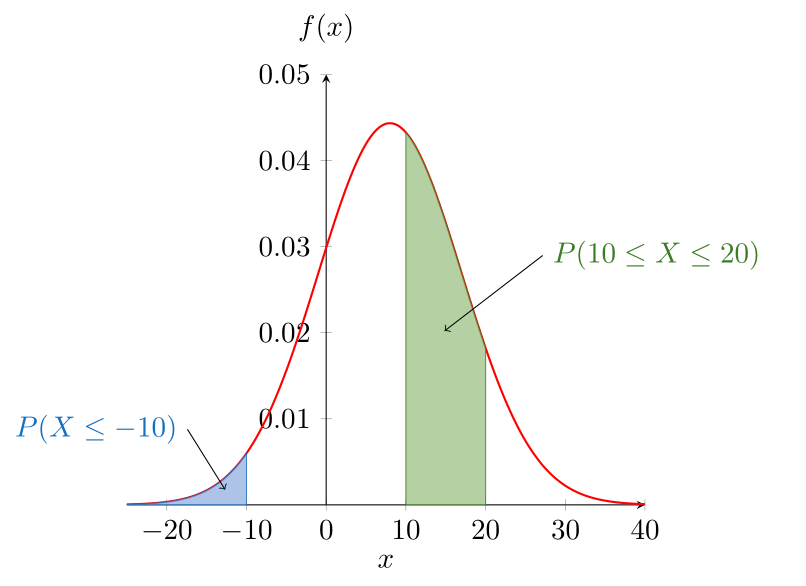
\includegraphics[width=0.7\linewidth]{img/p2} 

}

\caption{L'aire hachurée correspond à des probabilités. $f(x)$ étant une fonction densité de probabilité}\label{fig:p2}
\end{figure}

\BeginKnitrBlock{definition}
\protect\hypertarget{def:unnamed-chunk-33}{}{\label{def:unnamed-chunk-33} }Pour toute variable aléatoire continue \(X\) de densité \(f\):

\begin{itemize}
\item
  \(f(x) \ge 0 \quad \forall \, x \in \mathbb{R}\)
\item
  \(\int_{-\infty}^{+\infty}f(x)dx = 1\)
\item
  Si l'on pose \(a=b\) dans \eqref{eq:probab}, il résulte \[P(X=a)=\int_a^a f(x)dx = 0\]
\item
  Ceci siginifie que la probabilité qu'une variable aléatoire continue prenne une valeur isolée fixe est toujours nulle. Aussi on peut écrire

  \[P(X < a) = P( X \le a)  = \int_{-\infty}^a f(x)dx\]
\end{itemize}
\EndKnitrBlock{definition}

\BeginKnitrBlock{rmdexercise}
Soit \(X\) la variable aléatoire réelle de densité de probabilité

\[f(x)= \left\lbrace
      \begin{array}{ll}
      kx  & \mbox{si} \quad 0\le x \le 5\\
      0 & \mbox{sinon}
      \end{array}
  \right.\]

\begin{enumerate}
\def\labelenumi{\arabic{enumi}.}
\tightlist
\item
  Calculer \(k\).
\item
  Calculer: \(P(1 \le X \le 3), P(2 \le X \le 4)\) et \(P(X < 3)\).
\end{enumerate}
\EndKnitrBlock{rmdexercise}

\BeginKnitrBlock{rmdexercise}
Soit \(X\) une variable aléatoire réelle continue ayant pour densité de
probabilité \[f(x)= \left\lbrace
      \begin{array}{ll}
      \frac{1}{6} x + k  & \mbox{si} \quad 0\le x \le 3\\
      0 & \mbox{sinon}
      \end{array}
  \right.\]

\begin{enumerate}
\def\labelenumi{\arabic{enumi}.}
\tightlist
\item
  Calculer \(k\).
\item
  Calculer \(P(1 \le X \le 2)\)
\end{enumerate}
\EndKnitrBlock{rmdexercise}

\hypertarget{fonction-de-repartition-dune-v.a.c}{%
\section{Fonction de répartition d'une v.a.c}\label{fonction-de-repartition-dune-v.a.c}}

\BeginKnitrBlock{definition}
\protect\hypertarget{def:unnamed-chunk-36}{}{\label{def:unnamed-chunk-36} }Si comme pour les variables aléatoires discrètes, on définit la fonction
de répartition de \(X\) par:

\[\begin{aligned}
    F_X \colon  \mathbb{R} &\longrightarrow \mathbb{R} \\
                x &\longmapsto F_X(a) = P(X \le a)\end{aligned}\]

alors la relation entre la fonction de répartition \(F_X\) et la fonction
densité de probabilité \(f(x)\) est la suivante:

\[\forall \quad a \in \mathbb{R} \quad F_X(a)= P(X \le a) = \int_{-\infty}^a f(x)dx\]
\EndKnitrBlock{definition}

La fonction de répartition \(F_X(a)\) est la \textbf{primitive} de la fonction
densité de probabilité \(f(x)\) (donc la densité d'une v.a.c est la
dérivée de la fonction de répartition), et permet d'obtenir les
probabilités associées à la variable aléatoire \(X\), en effet:

\textbf{Propriétés:} Pour une variable aléatoire continue X:

\begin{itemize}
\item
  \(F'_X(x) = \frac{\text{d}}{\text{d} x} F_X(x) = f(x)\).
\item
  Pour tous réels \(a \le b\), \[\begin{aligned}
        P(a < X < b)      & = P(a < X \le b) \\
                          & = P(a \le X < b) \\
                          & = P( a \le X \le b) \\
                          & = F_X(b) - F_X(a) = \int_a^bf(x)dx
      \end{aligned}\]
\end{itemize}

La fonction de répartition correspond aux probabilités cumulées
associées à la variable aléatoire continue sur l'intervalle d'étude
(Figure \ref{fig:rep}).

\begin{figure}

{\centering 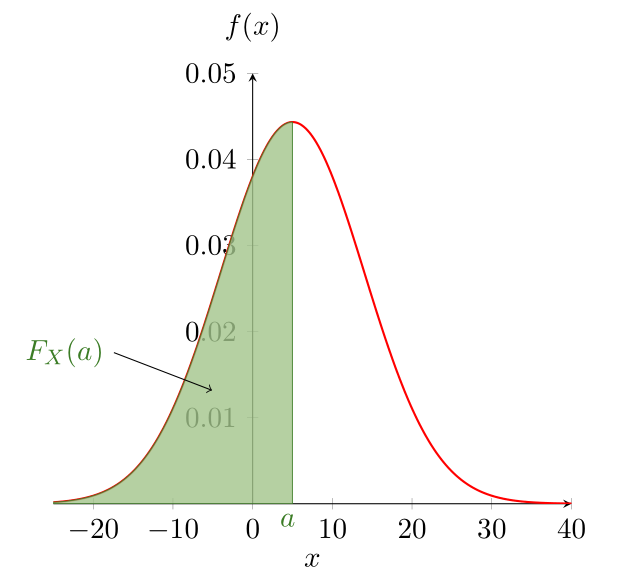
\includegraphics[width=0.7\linewidth]{img/rep} 

}

\caption{L'aire hachurée en vert sous la courbe de la fonction densité de probabilité correspond à la probabilité $P ( X < a ) = F_X ( a )$ et vaut 0.5 car ceci correspond exactement à la moitié de l'aire totale sous la courbe}\label{fig:rep}
\end{figure}

\textbf{Propriétés:} Les propriétés associées à la fonction de répartition sont les suivantes:

\begin{enumerate}
\def\labelenumi{\arabic{enumi}.}
\item
  \(F_X\) est continue sur \(\mathbb{R}\), dérivable en tout point où \(f\)
  est continue.
\item
  \(F_X\) est croissante sur \(\mathbb{R}\).
\item
  \(F_X\) est à valeurs dans \([0,1]\).
\item
  \(\lim\limits_{x\to - \infty} F_X(x) = 0\) et
  \(\lim\limits_{x\to +\infty} F_X(x) = 1\).
\end{enumerate}

\hypertarget{fonction-dune-variable-aleatoire-continue}{%
\section{Fonction d'une variable aléatoire continue}\label{fonction-dune-variable-aleatoire-continue}}

Soit \(X\) une variable aléatoire continue de densité \(f_X\) et de fonction
de répartition \(F_X\). Soit \(h\) une fonction continue définie sur
\(X(\Omega)\), alors \(Y=h(X)\) est une variable aléatoire.

Pour déterminer la densité de \(Y\), notée \(f_Y\), on commence par calculer
la fonction de répartition de \(Y\), notée \(F_Y\), ensuite nous dérivons
pour déterminer \(f_Y\).

\hypertarget{calcul-de-densites-pour-hxaxb}{%
\subsection*{\texorpdfstring{Calcul de densités pour \(h(X)=aX+b\)}{Calcul de densités pour h(X)=aX+b}}\label{calcul-de-densites-pour-hxaxb}}
\addcontentsline{toc}{subsection}{Calcul de densités pour \(h(X)=aX+b\)}

\(\forall \quad y \in \mathbb{R}\),

\[F_Y(y) = P(Y\leq y)=P(h(X) \le y) = P(aX+b \le y)\] si \(a>0\),
\[F_Y(y) = P(aX+b \le y) = P(X\leq \frac{y-b}{a})=F_X(\frac{y-b}{a})\]
si \(a<0\),
\[F_Y(y) = P(aX+b \le y) =P(X\geq \frac{y-b}{a})=1-F_X(\frac{y-b}{a})\]

En dérivant on obtient la densité de \(Y\)
\[f_Y(y)=\frac{1}{|a|}f_X(\frac{y-b}{a}).\]

\hypertarget{calcul-de-densites-pour-hxx2}{%
\subsection*{\texorpdfstring{Calcul de densités pour \(h(X)=X^2\)}{Calcul de densités pour h(X)=X\^{}2}}\label{calcul-de-densites-pour-hxx2}}
\addcontentsline{toc}{subsection}{Calcul de densités pour \(h(X)=X^2\)}

si \(y<0\), \(F_Y(y) =P(Y\leq y)=0\).\\
si \(y>0\),

\[F_Y(y) =P(Y\leq y)=P(X^2 \le y)=P(-\sqrt{y}\leq X \leq \sqrt{y})=F_X(\sqrt{y})-F_X(-\sqrt{y})\]

En dérivant on obtient la densité de \(Y\),

\[f_Y(y)= \left\lbrace
      \begin{array}{ll}
      \frac{1}{2\sqrt{y}}\big[f_X(\sqrt{y})+f_X(-\sqrt{y})\big]  & \mbox{si} \quad y \ge 0\\
      0 & \mbox{sinon}
      \end{array}
  \right.\]

\hypertarget{calcul-de-densites-pour-hxex}{%
\subsection*{\texorpdfstring{Calcul de densités pour \(h(X)=e^X\)}{Calcul de densités pour h(X)=e\^{}X}}\label{calcul-de-densites-pour-hxex}}
\addcontentsline{toc}{subsection}{Calcul de densités pour \(h(X)=e^X\)}

si \(y<0\), \(F_Y(y) = P(Y\leq y)=0\).\\
si \(y>0\),
\(F_Y(y) = P(Y\leq y)=P(e^X \le y)=P( X \leq \ln (y))=F_X(\ln(y))\).

En dérivant on obtient la densité de \(Y\)

\[f_Y(y)= \left\lbrace
      \begin{array}{ll}
      \frac{1}{y} f\big(\ln (y)\big)  & \mbox{si} \quad y \ge 0\\
      0 & \mbox{sinon}
      \end{array}
  \right.\]

\BeginKnitrBlock{rmdexercise}
Soit la v.a.c \(X\) ayant la
fonction de densité

\[f_X(x)= \left\lbrace
      \begin{array}{ll}
      2 x   & \mbox{si} \quad 0 \le x \le 1\\
      0 & \mbox{sinon}
      \end{array}
  \right.\]

Déterminer la densité de: \(Y=3X+1\), \(Z=X^2\) et \(T=e^X\).
\EndKnitrBlock{rmdexercise}

\hypertarget{esperance-et-variance-de-variables-aleatoires-continues}{%
\section{Espérance et variance de variables aléatoires continues}\label{esperance-et-variance-de-variables-aleatoires-continues}}

\hypertarget{esperance-dune-v.a.c}{%
\subsection*{Espérance d'une v.a.c}\label{esperance-dune-v.a.c}}
\addcontentsline{toc}{subsection}{Espérance d'une v.a.c}

\BeginKnitrBlock{definition}
\protect\hypertarget{def:unnamed-chunk-38}{}{\label{def:unnamed-chunk-38} }Si \(X\) est une variable aléatoire absolument continue de densité \(f\), on
appelle espérance de X, le réel \(E(X)\), défini par:

\[E(X)= \int_{-\infty}^{+\infty}x f(x) dx\] si cette intégrale est
convergente.
\EndKnitrBlock{definition}

Les propriétés de l'espérance d'une variable aléatoire continue sont les
mêmes que pour une variable aléatoire discrète.

\textbf{Propriétés:} Soit \(X\) une variable aléatoire continue,

\begin{itemize}
\item
  \(E(aX+b)=aE(X)+b \quad \quad a \ge 0 \,\, \text{et} \,\, b \in \mathbb{R}\).
\item
  Si \(X \ge 0\) alors \(E(X) \ge 0\).
\item
  Si \(X\) et \(Y\) sont deux variables aléatoires définies sur un même
  univers \(\Omega\) alors \[E(X+Y)=E(X)+E(Y)\]
\end{itemize}

\BeginKnitrBlock{theorem}[Théorème de transfert]
\protect\hypertarget{thm:transfert}{}{\label{thm:transfert} \iffalse (Théorème de transfert) \fi{} }Si \(X\) est une variable aléatoire de densité \(f(x)\), alors
pour toute fonction réelle \(g\) on aura

\[E[g(X)] = \int_{-\infty}^{+\infty}g(x) f(x) dx\]
\EndKnitrBlock{theorem}

\BeginKnitrBlock{rmdexercise}
Soit la v.a.c \(X\) ayant la fonction de densité

\[f_X(x)= \left\lbrace
      \begin{array}{ll}
      2 x   & \mbox{si} \quad 0 \le x \le 1\\
      0 & \mbox{sinon}
      \end{array}
  \right.\]

Calculer l'espérance des variables aléatoires \(Y=3X+1\),
\(Z=X^2\) et \(T=e^X\).
\EndKnitrBlock{rmdexercise}

\hypertarget{variance-dune-v.a.c}{%
\subsection*{Variance d'une v.a.c}\label{variance-dune-v.a.c}}
\addcontentsline{toc}{subsection}{Variance d'une v.a.c}

La variance d'une variable aléatoire \(V(X)\) est l'espérance mathématique
du carré de l'écart à l'espérance mathématique. C'est un paramètre de
dispersion qui correspond au moment centré d'ordre 2 de la variable
aléatoire \(X\).

\BeginKnitrBlock{definition}
\protect\hypertarget{def:unnamed-chunk-40}{}{\label{def:unnamed-chunk-40} }Si \(X\) est une variable aléatoire ayant une espérance \(E(X)\), on appelle
variance de \(X\) le réel

\[V(X)=E\big([X-E(X)]^2\big) = E(X^2) - [E(X)]^2\] Si \(X\) est une
variable aléatoire continue, on calcule \(E(X^2)\) en utilisant le
théorème \ref{thm:transfert},

\[E(X^2) = \int_{-\infty}^{+\infty}x^2 f(x)dx\]
\EndKnitrBlock{definition}

\textbf{Propriétés:} Si \(X\) est une variable aléatoire admettant une variance alors:

\begin{itemize}
\item
  \(V(X) \ge 0\), si elle existe.
\item
  \(\forall \quad a \in \mathbb{R}, V(aX) = a^2 V(X)\)
\item
  \(\forall \quad (a,b) \in \mathbb{R}, V(aX+b) = a^2 V(X)\)
\item
  Si \(X\) et \(Y\) sont deux variables aléatoires indépendantes,
  \(V(X+Y)=V(X)+V(Y)\)
\end{itemize}

\BeginKnitrBlock{definition}[Ecart-type]
\protect\hypertarget{def:unnamed-chunk-41}{}{\label{def:unnamed-chunk-41} \iffalse (Ecart-type) \fi{} }Si \(X\) est une variable aléatoire ayant une variance \(V(X)\), on appelle
écart-type de \(X\), le réel:

\[\sigma_X = \sqrt{V(X)}\]
\EndKnitrBlock{definition}

\hypertarget{lois-usuelles-de-v.a.c}{%
\section{Lois usuelles de v.a.c}\label{lois-usuelles-de-v.a.c}}

\hypertarget{loi-uniforme-uab}{%
\subsection*{\texorpdfstring{Loi uniforme \(U(a,b)\)}{Loi uniforme U(a,b)}}\label{loi-uniforme-uab}}
\addcontentsline{toc}{subsection}{Loi uniforme \(U(a,b)\)}

La loi uniforme est la loi exacte de phénomènes continus uniformément
répartis sur un intervalle.

\BeginKnitrBlock{definition}
\protect\hypertarget{def:unnamed-chunk-42}{}{\label{def:unnamed-chunk-42} }La variable aléatoire \(X\) suit une loi uniforme sur le segment \([a,b]\)
avec \(a < b\) si sa densité de probabilité est donnée par
\[f(x)= \left\lbrace
      \begin{array}{ll}
      \frac{1}{b-a}   & \mbox{si} \quad x \in [a,b]\\
      0 & \mbox{si} \quad x \notin [a,b]
      \end{array}
  \right. = \frac{1}{b-a} {1}_{[a,b]}(x)\]
\EndKnitrBlock{definition}

\begin{figure}

{\centering 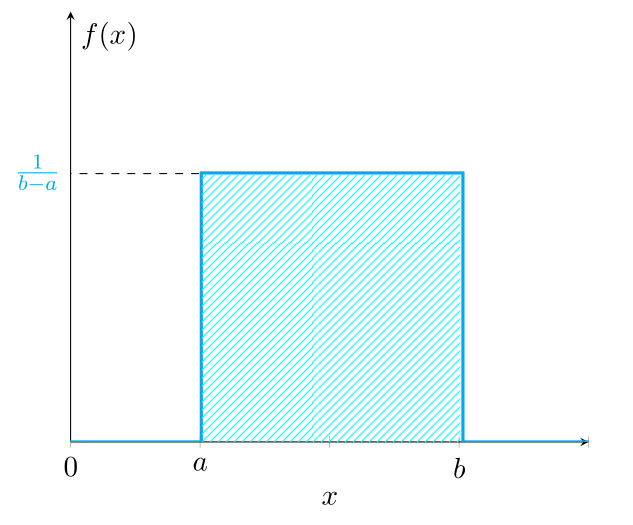
\includegraphics[width=0.7\linewidth]{img/unif} 

}

\caption{Fonction de densité de $U([a,b]$)}\label{fig:unif}
\end{figure}

\emph{Quelques commentaires:}

\begin{enumerate}
\def\labelenumi{\arabic{enumi}.}
\item
  La loi uniforme continue étant une loi de probabilité, l'aire hachurée en bleu sur la Figure \ref{fig:unif} vaut \(1\).
\item
  La fonction de répartition associée à la loi uniforme continue est
  \[F_X(x)= \left\lbrace
         \begin{array}{ll}
         0 & \mbox{si} \quad x < a \\
         \frac{x-a}{b-a}   & \mbox{si} \quad  a \le x \le b \\
         1 & \mbox{si} \quad x > b
         \end{array}
     \right.\]
\end{enumerate}

\textbf{Propriétés:} Si \(X\) est une v.a.c qui suit la loi uniforme sur \([a,b]\):

\begin{itemize}
\item
  \(E(X) = \frac{b+a}{2}\)
\item
  \(V(X) =\frac{(b-a)^2}{12}\)
\end{itemize}

\BeginKnitrBlock{rmdexercise}
Soit \(X \thicksim U(0,10)\). Calculer:

\begin{enumerate}
\def\labelenumi{\arabic{enumi}.}
\item
  \(P(X <3)\)
\item
  \(P(X\ge 6)\)
\item
  \(P(3 < X < 8)\)
\end{enumerate}
\EndKnitrBlock{rmdexercise}

\hypertarget{loi-exponentielle-mathcalelambda}{%
\subsection*{\texorpdfstring{Loi exponentielle \(\mathcal{E}(\lambda)\)}{Loi exponentielle \textbackslash mathcal\{E\}(\textbackslash lambda)}}\label{loi-exponentielle-mathcalelambda}}
\addcontentsline{toc}{subsection}{Loi exponentielle \(\mathcal{E}(\lambda)\)}

\BeginKnitrBlock{definition}
\protect\hypertarget{def:unnamed-chunk-44}{}{\label{def:unnamed-chunk-44} }On dit qu'une variable aléatoire \(X\) est \textbf{exponentielle} (ou suit la
loi exponentielle) de paramètre \(\lambda\) si sa densité est donnée par

\[f(x)= \left\lbrace
      \begin{array}{ll}
      \lambda e^{- \lambda x}   & \mbox{si} \quad x \ge 0\\
      0 & \mbox{si} \quad x < 0
      \end{array}
  \right. = \lambda e^{- \lambda x} {1}_{\mathbb{R}^{+}}(x)\]

On dit \(X \thicksim \mathcal{E}(\lambda)\)
\EndKnitrBlock{definition}

La fonction de répartition \(F\) d'une variable aléatoire exponentielle
est donnée par

\[\mbox{Si}\,\, x \ge 0 \quad F(x) = P(X \le x) = \int_0^x f(t)dt = \int_0^x \lambda e^{- \lambda t} dt  = \big[ -e^{- \lambda t} \big]_0^x = 1-e^{- \lambda x} \quad\]

\textbf{Propriétés:} Si \(X \thicksim \mathcal{E}(\lambda)\)

\begin{itemize}
\item
  \(E(X) = \frac{1}{\lambda}\)
\item
  \(V(X)= \frac{1}{\lambda^2}\)
\end{itemize}

\BeginKnitrBlock{rmdinsight}
\textbf{Cas d'utilisations de la loi exponentielle :} Dans la pratique, on
rencontre souvent la distribution exponentielle lorsqu'il s'agit de
représenter le temps d'attente avant l'arrivée d'un événement spécifié.
Une loi exponentielle modélise la durée de vie d'un phénomène sans
mémoire, ou sans vieillissement, ou sans usure. En d'autres termes, le
fait que le phénomène ait duré pendant un temps \(t\) ne change rien à son
espérance de vie à partir du temps \(t\). On dit qu'une variable aléatoire
non négative \(X\) est \textbf{sans mémoire} lorsque

\[P(X > t+h | X > t) = P(X > h) \quad \quad \forall \quad t,h \ge 0\]
Par exemple, la durée de vie de la radioactivité ou d'un composant
électronique, le temps qui nous sépare d'un prochain tremblement de
terre ou du prochain appel téléphonique mal aiguillé sont toutes des
variables aléatoires dont les distributions tendent en pratique à se
rapprocher de distributions exponentielles.
\EndKnitrBlock{rmdinsight}

\hypertarget{loi-normale-ou-de-laplace-gauss-mathcalnmusigma2}{%
\subsection*{\texorpdfstring{Loi Normale ou de Laplace-Gauss \(\mathcal{N}(\mu,\sigma^2)\)}{Loi Normale ou de Laplace-Gauss \textbackslash mathcal\{N\}(\textbackslash mu,\textbackslash sigma\^{}2)}}\label{loi-normale-ou-de-laplace-gauss-mathcalnmusigma2}}
\addcontentsline{toc}{subsection}{Loi Normale ou de Laplace-Gauss \(\mathcal{N}(\mu,\sigma^2)\)}

\BeginKnitrBlock{definition}
\protect\hypertarget{def:unnamed-chunk-46}{}{\label{def:unnamed-chunk-46} }Une variable aléatoire \(X\) est dite \textbf{normale} avec paramètres \(\mu\) et
\(\sigma^2\) si la densité de \(X\) est donnée par

\[f(x) = \frac{1}{\sigma \sqrt{2\pi}} e^{-(x - \mu)^2/2\sigma^2} \quad \quad \forall \,\, x \in \mathbb{R}\]

Avec \(\mu \in \mathbb{R}\) et \(\sigma \in \mathbb{R}^{+}\). On dit que
\(X \thicksim \mathcal{N}(\mu,\sigma^2)\).
\EndKnitrBlock{definition}

\textbf{Remarque:} On admet que \(\int_{-\infty}^{+\infty}f(x)dx = 1\) dans la mesure où l'intégration analytique est impossible.

\hypertarget{etude-de-la-densite-de-la-loi-normale}{%
\subsection*{Étude de la densité de la loi Normale}\label{etude-de-la-densite-de-la-loi-normale}}
\addcontentsline{toc}{subsection}{Étude de la densité de la loi Normale}

\begin{itemize}
\item
  La fonction \(f\) est paire autour d'un axe de symétrie \(x = \mu\) car
  \(f(x + \mu ) = f(\mu - x)\).
\item
  \(f'(x)=0\) pour \(x=\mu\), \(f'(x) < 0\) pour \(x < \mu\) et \(f'(x) > 0\)
  pour \(x > \mu\)
\end{itemize}

\begin{figure}

{\centering 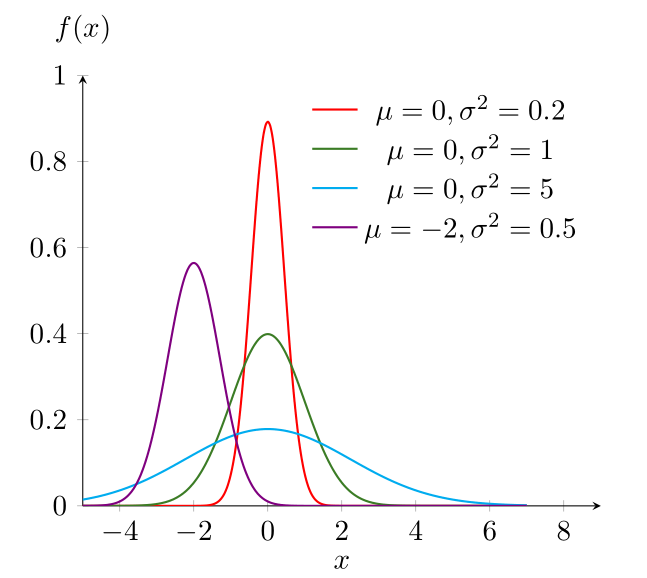
\includegraphics[width=0.7\linewidth]{img/norm} 

}

\caption{Représentation graphique de la densité d’une loi normale. Remarque: Le paramètre $\mu$ représente l’axe de symétrie et s le degré d’aplatissement de la courbe de la loi normale dont la forme est celle d’une courbe en cloche}\label{fig:norm}
\end{figure}

\textbf{Propriétés:} Soit \(X \thicksim \mathcal{N}(\mu,\sigma^2)\), on a:

\begin{itemize}
\tightlist
\item
  \(E(X)=\mu\)
\item
  \(V(X)=\sigma^2\)
\end{itemize}

\BeginKnitrBlock{theorem}[Stabilité de la loi normale]
\protect\hypertarget{thm:unnamed-chunk-47}{}{\label{thm:unnamed-chunk-47} \iffalse (Stabilité de la loi normale) \fi{} }Soit \(X_1\) et \(X_2\) deux variables
aléatoires normales et indépendantes de paramètres respectifs
\((\mu_1,\sigma_1^2)\) et \((\mu_2,\sigma_2^2)\), alors leur somme \(X_1+X_2\)
est une variable aléatoire normale de paramètres
\((\mu_1 + \mu_2,\sigma_1^2+\sigma_2^2)\).
\EndKnitrBlock{theorem}

\hypertarget{loi-normale-centree-reduite-mathcaln01}{%
\subsection*{\texorpdfstring{Loi Normale centrée réduite \(\mathcal{N}(0,1)\)}{Loi Normale centrée réduite \textbackslash mathcal\{N\}(0,1)}}\label{loi-normale-centree-reduite-mathcaln01}}
\addcontentsline{toc}{subsection}{Loi Normale centrée réduite \(\mathcal{N}(0,1)\)}

\BeginKnitrBlock{definition}
\protect\hypertarget{def:unnamed-chunk-48}{}{\label{def:unnamed-chunk-48} }Une variable aléatoire continue \(X\) suit une \textbf{loi normale centrée
réduite} si sa densité de probabilité est donnée par

\begin{equation}
f(x) =  \frac{1}{{\sqrt {2\pi } }}e^{- \frac{1}{2} x^2} \quad \quad \forall \,\, x \in \mathbb{R}
\end{equation}

On dit \(X \thicksim \mathcal{N}(0,1)\).
\EndKnitrBlock{definition}

\textbf{Remarque:} \(E(X)=0\) et \(V(X)=1\).

\begin{figure}

{\centering 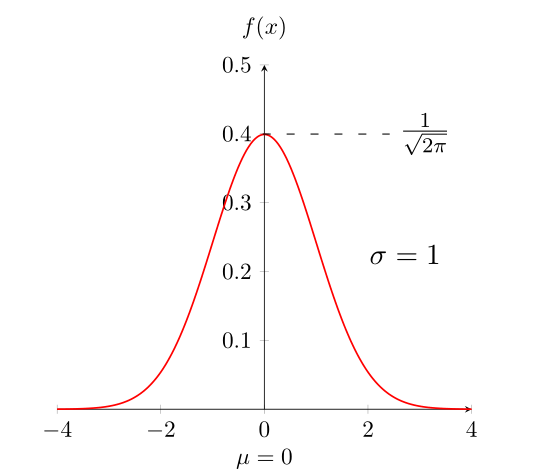
\includegraphics[width=0.5\linewidth]{img/normcr} 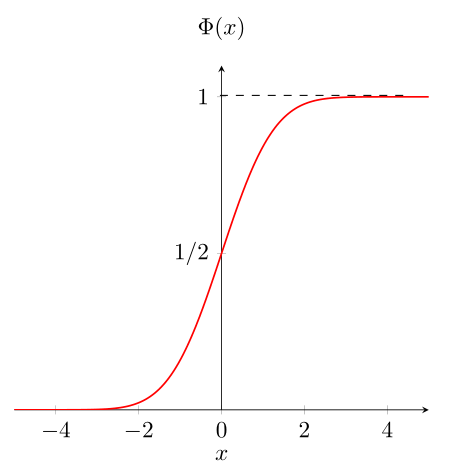
\includegraphics[width=0.5\linewidth]{img/phi} 

}

\caption{(gauche): Densité d'une loi normale centrée réduite $\mathcal{N}(0,1)$. (droite): Fonction de répartition de $\mathcal{N}(0,1)$.}\label{fig:normal}
\end{figure}

\hypertarget{relation-entre-loi-normale-et-loi-normale-centree-reduite}{%
\subsection*{Relation entre loi normale et loi normale centrée réduite}\label{relation-entre-loi-normale-et-loi-normale-centree-reduite}}
\addcontentsline{toc}{subsection}{Relation entre loi normale et loi normale centrée réduite}

\BeginKnitrBlock{theorem}[Relation avec la loi normale]
\protect\hypertarget{thm:unnamed-chunk-49}{}{\label{thm:unnamed-chunk-49} \iffalse (Relation avec la loi normale) \fi{} }Si \(X\) suit une loi normale
\(\mathcal{N}(\mu,\sigma^2)\), alors \(Z= \frac{X-\mu}{\sigma}\) est une
variable centrée réduite qui suit la loi normale centrée réduite
\(\mathcal{N}(0,1)\).
\EndKnitrBlock{theorem}

\hypertarget{calcul-des-probabilites-dune-loi-normale}{%
\subsection*{Calcul des probabilités d'une loi normale}\label{calcul-des-probabilites-dune-loi-normale}}
\addcontentsline{toc}{subsection}{Calcul des probabilités d'une loi normale}

La fonction de répartition de la loi normale réduite permet d'obtenir
les probabilités associées à toutes variables aléatoires normales
\(\mathcal{N}(\mu,\sigma^2)\) après transformation en variable centrée
réduite.

\BeginKnitrBlock{definition}
\protect\hypertarget{def:unnamed-chunk-50}{}{\label{def:unnamed-chunk-50} }On appelle fonction \(\Phi\), la fonction de répartition de la loi normale
centrée réduite \(\mathcal{N}(0,1)\), telle que

\[\forall \,\, x \in \mathbb{R} \quad \Phi(x) = P(X \le x) =  \frac{1}{{\sqrt {2\pi}}} \int_{-\infty}^x f(t)dt\]
\EndKnitrBlock{definition}

\textbf{Propriétés:} Les propriétés associées à la fonction de répartition \(\Phi\) sont:

\begin{enumerate}
\def\labelenumi{\arabic{enumi}.}
\item
  \(\Phi\) est croissante, continue et dérivable sur \(\mathbb{R}\) et
  vérifie:

  \(\lim\limits_{x\to - \infty} \Phi(x) = 0\) et
  \(\lim\limits_{x\to\infty} \Phi(x) = 1\)
\item
  \(\forall \,\, x \in \mathbb{R} \quad \Phi(x) + \Phi(-x) = 1\)
\item
  \(\forall \,\, x \in \mathbb{R} \quad \Phi(x) - \Phi(-x) = 2\Phi(x) -1\)
\end{enumerate}

Une application directe de la fonction \(\Phi\) est la lecture des
probabilités de la loi normale sur la table de la loi normale centrée
réduite.

\BeginKnitrBlock{rmdexercise}
Soit \(X\) une variable aléatoire normale de paramètres \(\mu =3\) et
\(\sigma^2=4\). Calculer:

\begin{enumerate}
\def\labelenumi{\arabic{enumi}.}
\item
  \(P(X > 0)\)
\item
  \(P(2 < X < 5)\)
\item
  \(P(|X-3| > 4)\)
\end{enumerate}
\EndKnitrBlock{rmdexercise}

\hypertarget{approximation-normale-dune-repartition-binomiale}{%
\subsection*{Approximation normale d'une répartition binomiale}\label{approximation-normale-dune-repartition-binomiale}}
\addcontentsline{toc}{subsection}{Approximation normale d'une répartition binomiale}

Un résultat important de la théorie de probabilité est connu sous le nom
de théorème limite de Moivre-Laplace. Il dit que pour \(n\) grand, une
variable binomiale \(\mathcal{B}(n,p)\) suivra approximativement la même
loi qu'une variable aléatoire normale avec même moyenne et même
variance. Ce théorème énonce que si ``on standardise'' une variable
aléatoire binomiale \(\mathcal{B}(n,p)\) en soustrayant d'abord sa moyenne
\(np\) puis en divisant le résultat par son écart-type \(\sqrt{np(1-p)}\),
alors la variable aléatoire standardisée (de moyenne 0 et variance 1)
suivra approximativement, lorsque \(n\) est grand, une distribution
normale standard. Ce résultat fut ensuite progressivement généralisé par
Laplace, Gauss et d'autres pour devenir le théorème actuellement connu
comme théorème centrale limite qui est un des deux résultats les plus
importants de la théorie de probabilités. Ce théorème sert de base
théorique pour expliquer un fait empirique souvent relevé, à savoir
qu'en pratique de très nombreux phénomènes aléatoires suivent
approximativement une distribution normale.

On remarquera qu'à ce stade deux approximations de la répartition
binomiale ont été proposées: l'approximation de Poisson, satisfaisante
lorsque \(n\) est grand et lorsque \(np\) n'est pas extrême; l'approximation
normale pour laquelle on peut montrer qu'elle est de bonne qualité
lorsque \(np(1-p)\) est grand (dès que \(np(1-p)\) dépasse 10).

\begin{figure}

{\centering 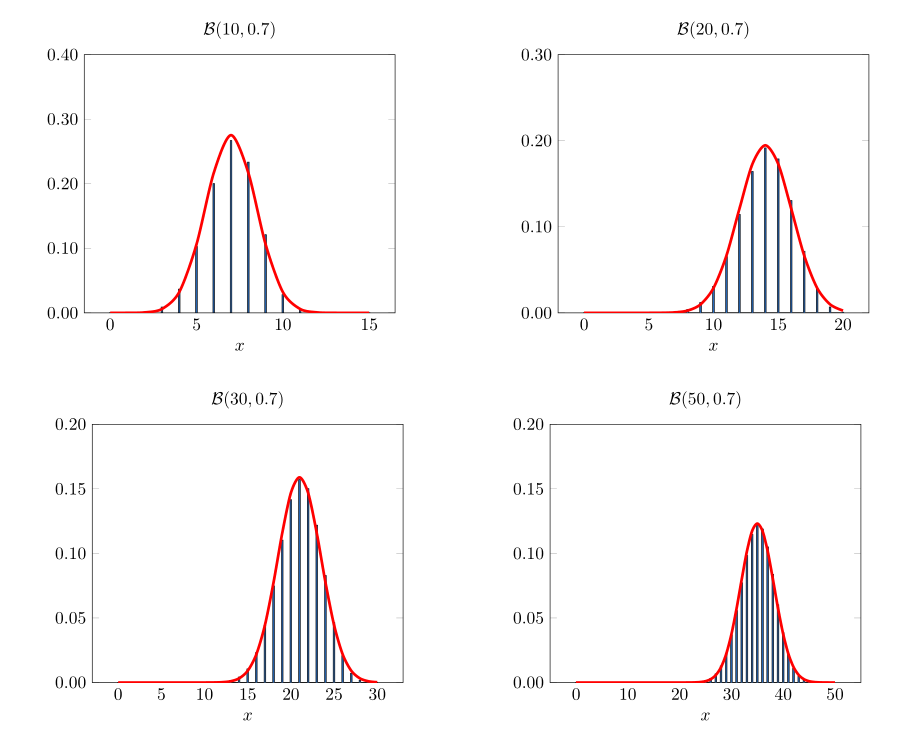
\includegraphics[width=0.7\linewidth]{img/binomnorm} 

}

\caption{La loi de probabilité d’une variable aléatoire $B( n,p )$ devient de plus en plus **normale** à mesure que $n$ augmente.}\label{fig:binomnorm}
\end{figure}

\hypertarget{loi-de-chi2-de-pearson}{%
\subsection*{\texorpdfstring{Loi de \(\chi^{2}\) de Pearson}{Loi de \textbackslash chi\^{}\{2\} de Pearson}}\label{loi-de-chi2-de-pearson}}
\addcontentsline{toc}{subsection}{Loi de \(\chi^{2}\) de Pearson}

\BeginKnitrBlock{definition}
\protect\hypertarget{def:unnamed-chunk-52}{}{\label{def:unnamed-chunk-52} }Soit \(X_1,X_2,\ldots,X_n\), \(n\) variables \textbf{normales centrées réduites},
et \(Y\) la variable aléatoire définie par

\[Y = X_1^2 + X_2^2 + \ldots + X_i^2 + \ldots + X_n^2 = \sum_{i=1}^n X_i^2\]
On dit que \(Y\) suit la loi de \(\chi^2\) (ou loi de Pearson) à \(n\) degrés
de liberté, \(Y \thicksim \chi^2 (n)\)
\EndKnitrBlock{definition}

\BeginKnitrBlock{rmdinsight}
La loi de \(\chi^2\) trouve de nombreuses applications dans le cadre de la
comparaison de proportions, des tests de conformité d'une distribution
observée à une distribution théorique et le test d'indépendance de deux
caractères qualitatifs. Ce sont les \emph{tests du khi-deux}.
\EndKnitrBlock{rmdinsight}

\textbf{Remarque:} Si \(n=1\), la variable du \(\chi^2\) correspond au carré d'une variable normale centrée réduite \(\mathcal{N}(0,1)\).

\textbf{Propriétés:} Si \(Y \thicksim \chi^2 (n)\), alors:

\begin{itemize}
\item
  \(E(Y)= n\)
\item
  \(V(Y) = 2n\)
\end{itemize}

\hypertarget{loi-de-student-stn}{%
\subsection*{\texorpdfstring{Loi de Student \(St(n)\)}{Loi de Student St(n)}}\label{loi-de-student-stn}}
\addcontentsline{toc}{subsection}{Loi de Student \(St(n)\)}

\BeginKnitrBlock{definition}
\protect\hypertarget{def:unnamed-chunk-54}{}{\label{def:unnamed-chunk-54} }Soit \(U\) une variable aléatoire suivant une loi \textbf{normale centrée
réduite} \(\mathcal{N}(0,1)\) et \(V\) une variable aléatoire suivant une
loi de \(\chi^2(n)\), \(U\) et \(V\) étant indépendantes, on dit alors que
\(T_n = \frac{U}{\sqrt{\frac{V}{n}}}\) suit une \textbf{loi de Student} à \(n\)
degrés de liberté. \(T_n \thicksim St(n)\)
\EndKnitrBlock{definition}

\BeginKnitrBlock{rmdinsight}
La loi de Student est utilisée lors des tests de comparaison de
paramètres comme la moyenne et dans l'estimation de paramètres de la
population à partir de données sur un échantillon (Test de Student).
\EndKnitrBlock{rmdinsight}

\hypertarget{loi-de-fisher-snedecor-mathcalfnm}{%
\subsection*{\texorpdfstring{Loi de Fisher-Snedecor \(\mathcal{F}(n,m)\)}{Loi de Fisher-Snedecor \textbackslash mathcal\{F\}(n,m)}}\label{loi-de-fisher-snedecor-mathcalfnm}}
\addcontentsline{toc}{subsection}{Loi de Fisher-Snedecor \(\mathcal{F}(n,m)\)}

\BeginKnitrBlock{definition}
\protect\hypertarget{def:unnamed-chunk-56}{}{\label{def:unnamed-chunk-56} }Soit \(U\) et \(V\) deux variables aléatoires indépendantes suivant une loi
de \(\chi^2\) respectivement à \(n\) et \(m\) degrés de liberté.

On dit que \(F= \frac{U/n}{V/m}\) suit une loi de Fisher-Snedecor à
\((n,m)\) degrés de liberté. \(F \thicksim \mathcal{F}(n,m)\)
\EndKnitrBlock{definition}

\BeginKnitrBlock{rmdinsight}
La loi de Fisher-Snedecor est utilisée pour comparer deux variances
observées et sert surtout dans les très nombreux tests d'analyse de
variance et de covariance.
\EndKnitrBlock{rmdinsight}

\hypertarget{couple-de-variables-aleatoires-continues}{%
\section{Couple de variables aléatoires continues}\label{couple-de-variables-aleatoires-continues}}

\hypertarget{densite-conjointe}{%
\subsection*{Densité conjointe}\label{densite-conjointe}}
\addcontentsline{toc}{subsection}{Densité conjointe}

\BeginKnitrBlock{definition}
\protect\hypertarget{def:unnamed-chunk-58}{}{\label{def:unnamed-chunk-58} }On dit que \((X,Y)\) est un couple aléatoire continu s'il existe une
fonction \(f: \mathbb{R}^2 \rightarrow \mathbb{R}\) telle que pour tout
\(D \subseteq \mathbb{R}\) on a

\[P\{(X,Y) \in D\} = \iint\limits_{(x,y) \in D} f(x,y) dx dy\]
\EndKnitrBlock{definition}

\textbf{Remarque:} On a la condition de normalité
\(\iint\limits_{\mathbb{R}^2} f(x,y)dxdy=1\)

La fonction \(f\) s'appelle \textbf{densité conjointe} de \(X\) et \(Y\). Notons
par \(A\) et \(B\) deux ensembles de nombres réels. En définissant
\(D=\{(x,y) : x \in A, y \in B\}\), on obtient

\[P(X\in A, Y \in B) = \int_A \int_B f(x,y) dxdy\]

La fonction de répartition du \((X,Y)\) est définie par

\[F(a,b)=P(X \le a, Y \le b) = \int_{- \infty}^b \int_{- \infty}^a  f(x,y) dx dy\]

\(f\) est le dérivé de \(F\):
\(f(a,b)= \frac{\partial^2}{\partial a \partial b} F(a,b)\)

\BeginKnitrBlock{rmdexercise}
Soit \((X,Y)\) un couple
aléatoire continu de densité \[f(x,y)= \left\lbrace
      \begin{array}{ll}
      a x y^2   & \mbox{si} \quad 0 \le x \le y \le 1 \\
      0 & \mbox{sinon}
      \end{array}
  \right.\] Trouver la constante \(a\).
\EndKnitrBlock{rmdexercise}

\BeginKnitrBlock{rmdexercise}
Soit \((X,Y)\) un couple
aléatoire continu de densité

\[f(x,y)= \left\lbrace
      \begin{array}{ll}
      2 e^{-x} e^{-2y}   & \mbox{si} \quad x > 0, \,\, y > 0\\
      0 & \mbox{sinon}
      \end{array}
  \right.\] Montrer que:

\begin{enumerate}
\def\labelenumi{\arabic{enumi}.}
\item
  \(P(X > 1, Y < 1)=e^{-1}(1-e^{-2})\)
\item
  \(P(X < a) = 1-e^{-a}\)
\item
  \(P(X < Y ) = 1/3\)
\end{enumerate}
\EndKnitrBlock{rmdexercise}

\hypertarget{densites-marginales}{%
\subsection*{Densités marginales}\label{densites-marginales}}
\addcontentsline{toc}{subsection}{Densités marginales}

Si on dispose de la densité du couple, on peut retrouver les densités de
\(X\) et de \(Y\), appelées les densités marginales:

\textbf{Densité marginale de X:} \[f(x,.)=f_X(x)=\int_{\mathbb{R}} f(x,y)dy\]

\textbf{Densité marginale de Y:} \[f(.,y)=f_Y(y)=\int_{\mathbb{R}} f(x,y)dx\]

\hypertarget{esperance-dune-fonction-du-couple}{%
\subsection*{Espérance d'une fonction du couple}\label{esperance-dune-fonction-du-couple}}
\addcontentsline{toc}{subsection}{Espérance d'une fonction du couple}

Si \((X,Y)\) est un couple continu de densité \(f(x,y)\) et
\(g: \mathbb{R}^2 \rightarrow \mathbb{R}\) on a

\[E[ g(X,Y)] =  \iint\limits_{\mathbb{R}^2} g(x,y) f(x,y)dxdy\]

\hypertarget{independance}{%
\subsection*{Indépendance}\label{independance}}
\addcontentsline{toc}{subsection}{Indépendance}

Les v.a. \(X\) et \(Y\) sont indépendantes ssi
\(\forall \, (x,y) \in \mathbb{R}^2\) on a

\[f(x,y)=f_X(x) f_Y(y)\]

\hypertarget{distribution-conditionnelle}{%
\subsection*{Distribution conditionnelle}\label{distribution-conditionnelle}}
\addcontentsline{toc}{subsection}{Distribution conditionnelle}

Si \((X,Y)\) est un couple continu de densité \(f(x,y)\), on définit
\textbf{densité conditionnelle de \(X\)}, sous la condition \(Y=y\) et lorsque
\(f_Y(y) > 0\) par la relation

\[f_{X|Y} (x|y) = \frac{f(x,y)}{f_Y(y)}\]

\BeginKnitrBlock{rmdexercise}
Supposons que \(X\) et \(Y\) aient pour densité conjointe
\[f(x,y)= \left\lbrace
      \begin{array}{ll}
      \frac{1}{y} e^{- x/y}e^{-y}   & \mbox{si} \quad x > 0, \,\, y > 0\\
      0 & \mbox{sinon}
      \end{array}
  \right.\]

\begin{enumerate}
\def\labelenumi{\arabic{enumi}.}
\item
  Déterminer la densité conditionnelle de \(X\) lorsque \(Y=y\).
\item
  Calculer \(P(X>1 | Y = y)\)
\end{enumerate}
\EndKnitrBlock{rmdexercise}

\hypertarget{exercices}{%
\chapter*{Exercices}\label{exercices}}
\addcontentsline{toc}{chapter}{Exercices}

\hypertarget{combinatoire}{%
\section*{Combinatoire}\label{combinatoire}}
\addcontentsline{toc}{section}{Combinatoire}

\BeginKnitrBlock{exercise}
\protect\hypertarget{exr:unnamed-chunk-63}{}{\label{exr:unnamed-chunk-63} }On tire simultanément 5 cartes d'un jeu de 52 cartes.

\begin{enumerate}
\def\labelenumi{\arabic{enumi}.}
\item
  Combien de tirages différents peut-on obtenir?
\item
  Combien de tirages peut-on obtenir ? contenant:

  \begin{enumerate}
  \def\labelenumii{\arabic{enumii}.}
  \item
    5 carreaux ou 5 coeurs;
  \item
    2 coeurs et 3 piques;
  \item
    au moins 1 roi;
  \item
    au plus 1 roi.
  \end{enumerate}
\end{enumerate}
\EndKnitrBlock{exercise}

\BeginKnitrBlock{exercise}
\protect\hypertarget{exr:unnamed-chunk-64}{}{\label{exr:unnamed-chunk-64} }On jette un dé équilibré 3 fois de suite, et on s'intéresse au total des
points obtenus. De combien de façons peut-on obtenir:

\begin{enumerate}
\def\labelenumi{\arabic{enumi}.}
\item
  un total égale à 16.
\item
  un total égale à 15.
\item
  un total au moins égale à 15.
\end{enumerate}
\EndKnitrBlock{exercise}

\hypertarget{evenements}{%
\section*{Événements}\label{evenements}}
\addcontentsline{toc}{section}{Événements}

\BeginKnitrBlock{exercise}
\protect\hypertarget{exr:unnamed-chunk-65}{}{\label{exr:unnamed-chunk-65} }Soit \(A\),\(B\) et \(C\) trois événements d'un espace probabilisable
\((\Omega,\mathcal{A})\). Exprimer en fonction de \(A\),\(B\) et \(C\) et des
opérations ensemblistes (réunion, intersection et complémentaire) les
événements ci-après:

\begin{enumerate}
\def\labelenumi{\arabic{enumi}.}
\item
  \(A\) seul (parmi les 3 événements) se produit.
\item
  \(A\) et \(C\) se produisent, mais non \(B\).
\item
  Les trois événements se produisent.
\item
  L'un au moins des 3 événements se produit.
\item
  Aucun des trois événements ne se produit.
\item
  Deux événements exactement se produisent.
\item
  Pas plus de deux événements ne se produisent.
\end{enumerate}
\EndKnitrBlock{exercise}

\hypertarget{probabilite}{%
\section*{Probabilité}\label{probabilite}}
\addcontentsline{toc}{section}{Probabilité}

\BeginKnitrBlock{exercise}
\protect\hypertarget{exr:unnamed-chunk-66}{}{\label{exr:unnamed-chunk-66} }Soit \((\Omega,\mathcal{A},P)\) un espace probabilisé. Soient \(A\),\(B\) et \(C\)
trois événements quelconques. On pose :
\(E = A \cap \bar{B} \cap \bar{C}\) et \(F = A \cap (B \cup C)\).

\begin{enumerate}
\def\labelenumi{\arabic{enumi}.}
\item
  Montrer que \(E\) et \(F\) sont incompatibles.
\item
  Montrer que \(E \cup F = A\).
\item
  Sachant que \(P(A)=0.6; \, P(A\cap B)=0.2; \, P(A\cap C)=0.1\) et
  \(P(A\cap B \cap C)=0.05\): Calculer \(P(F)\) et \(P(E)\).
\end{enumerate}
\EndKnitrBlock{exercise}

\hypertarget{variables-aleatoires-discretes-2}{%
\section*{Variables aléatoires discrètes}\label{variables-aleatoires-discretes-2}}
\addcontentsline{toc}{section}{Variables aléatoires discrètes}

\BeginKnitrBlock{exercise}
\protect\hypertarget{exr:unnamed-chunk-67}{}{\label{exr:unnamed-chunk-67} }On choisit deux boules au hasard dans une urne contenant 8 boules
blanches, 4 boules noires et 2 boules oranges. Supposons que l'on
reçoive 2 euros pour chaque boule noire tirée et que l'on perde 1 euro
pour chaque boule blanche tirée. Désignons les gains nets par X.

\begin{enumerate}
\def\labelenumi{\arabic{enumi}.}
\item
  Quelles sont les valeurs possibles pour X et les probabilités
  associées à ces valeurs ?
\item
  Quelle est l'espérance de X ?
\end{enumerate}
\EndKnitrBlock{exercise}

\BeginKnitrBlock{exercise}
\protect\hypertarget{exr:unnamed-chunk-68}{}{\label{exr:unnamed-chunk-68} }Une urne contient une boule qui porte le numéro 0, deux qui portent le
numéro 1 et quatre qui portent le numéro 3. On extrait simultanément
deux boules dans cette urne.

\begin{enumerate}
\def\labelenumi{\arabic{enumi}.}
\item
  Déterminer la loi de probabilité de la variable aléatoire \(X\) qui
  représente la somme des nombres obtenus.
\item
  Déterminer la fonction de répartition de \(X\).
\item
  Calculer \(E(X)\), \(V(X)\) et \(\sigma(X)\).
\end{enumerate}
\EndKnitrBlock{exercise}

\BeginKnitrBlock{exercise}
\protect\hypertarget{exr:unnamed-chunk-69}{}{\label{exr:unnamed-chunk-69} }Soit \(X\) une v.a. qui suit la loi uniforme (e.g.~équiprobabilité de
valeurs de \(X\)) sur l'ensemble \(X(\Omega) = \{-3, -2, 1, 4\}\).

\begin{enumerate}
\def\labelenumi{\arabic{enumi}.}
\item
  Donner la loi de \(X\).
\item
  Calculer \(E(X)\) et \(V(X)\).

  On définit la variable aléatoire \(Y=(X+1)^2\).
\item
  Donner \(Y(\Omega)\) et la loi de \(Y\).
\item
  Calculer \(E(Y)\) de deux façons différents.
\end{enumerate}
\EndKnitrBlock{exercise}

\BeginKnitrBlock{exercise}
\protect\hypertarget{exr:unnamed-chunk-70}{}{\label{exr:unnamed-chunk-70} }Soient X et Y des variables aléatoires discrètes dont la loi jointe est
donnée par le tableau suivant:

\begin{longtable}[]{@{}ccccc@{}}
\toprule
\(X\)\textbackslash{}\(Y\) & -1 & 0 & 2 & 5\tabularnewline
\midrule
\endhead
0 & 0.10 & 0.05 & 0.15 & 0.05\tabularnewline
1 & 0.15 & 0.20 & 0.25 & 0.05\tabularnewline
\bottomrule
\end{longtable}

\begin{enumerate}
\def\labelenumi{\arabic{enumi}.}
\item
  Quelle est la loi marginale de X ?
\item
  Quelle est la loi marginale de Y ?
\item
  Calculer \(P(Y \geq 0 / X = 1)\).
\item
  Calculer \(E(X)\), \(E(Y)\), et \(cov(X,Y)\).
\item
  Les variables \(X\) et \(Y\) sont elles indépendantes ?
\end{enumerate}
\EndKnitrBlock{exercise}

\BeginKnitrBlock{exercise}
\protect\hypertarget{exr:unnamed-chunk-71}{}{\label{exr:unnamed-chunk-71} }Soit \((X,Y)\) un couple de variables aléatoires à valeurs dans
\(\mathbb{N}^2\) tel que

\[\forall (p,q) \in \mathbb{N}^2, \quad P(X=p,Y=q) = \lambda \frac{p+q}{p! q! 2^{p+q}}\]

\begin{enumerate}
\def\labelenumi{\arabic{enumi}.}
\item
  Déterminer \(\lambda\).
\item
  Calculer les lois marginales.
\item
  Les variables \(X\) et \(Y\) sont elles indépendantes ?
\end{enumerate}
\EndKnitrBlock{exercise}

\BeginKnitrBlock{exercise}
\protect\hypertarget{exr:unnamed-chunk-72}{}{\label{exr:unnamed-chunk-72} }Une urne contient 2 boules de numéro 20, 4 boules de numéro 10 et 4
boules de numéro 5.

\begin{enumerate}
\def\labelenumi{\arabic{enumi}.}
\item
  Une épreuve consiste à tirer simultanément 3 boules de l'urne.
  Calculer la probabilité \(p\) que la somme des numéros tirés soit
  égale à 30.
\item
  On répéte cette épreuve 4 fois en remettant à chaque fois les trois
  boules tirés dans l'urne. Soit \(X\) la v.a. indiquant le nombre de
  tirages donnant une somme de numéros égale à 30.

  \begin{enumerate}
  \def\labelenumii{\arabic{enumii}.}
  \item
    Quelle la loi de \(X\). Donner son espérance et son écart-type.
  \item
    Déterminer la probabilité d'avoir au moins une fois la somme 30
    dans les 4 tirages.
  \end{enumerate}
\end{enumerate}
\EndKnitrBlock{exercise}

\BeginKnitrBlock{exercise}
\protect\hypertarget{exr:unnamed-chunk-73}{}{\label{exr:unnamed-chunk-73} }Vous avez besoin d'une personne pour vous aider à déménager. Quand vous
téléphonez à un ami, il y a une chance sur quatre qu'il accepte. Soit
\(X\) la variable aléatoire qui représente le nombre d'amis que vous
devrez contacter pour obtenir cette aide.

\begin{enumerate}
\def\labelenumi{\arabic{enumi}.}
\item
  Déterminer la loi de probabilité de \(X\).
\item
  Calculer \(P(X\leq 3)\).
\item
  Calculer \(E(X)\).
\end{enumerate}
\EndKnitrBlock{exercise}

\BeginKnitrBlock{exercise}
\protect\hypertarget{exr:unnamed-chunk-74}{}{\label{exr:unnamed-chunk-74} }Pour être sélectionné aux jeux olympiques, un athlète doit réussir deux
fois à dépasser les minima fixés par sa fédération. Il a une chance sur
trois de réussir à chaque épreuve à laquelle il participe. On note \(X\)
la variable aléatoire qui représente le nombre d'épreuves auxquelles il
devra participer pour être sélectionné.

\begin{enumerate}
\def\labelenumi{\arabic{enumi}.}
\item
  Déterminer la loi de probabilité de \(X\).
\item
  Si cet athlète ne peut participer qu'à quatre épreuves maximum,
  quelle est la probabilité qu'il soit sélectionné ?
\end{enumerate}
\EndKnitrBlock{exercise}

\BeginKnitrBlock{exercise}
\protect\hypertarget{exr:unnamed-chunk-75}{}{\label{exr:unnamed-chunk-75} }Un sac contient cinq jetons : deux sont numérotés 1 et les trois autres
sont numérotés 2. On effectue une série illimitée de tirages avec remise
d'un jeton dans le sac S. On désigne par \(Y\) la variable aléatoire égale
au nombre de tirages effectués avant le tirage amenant un jeton numéroté
1 pour la première fois.

\begin{enumerate}
\def\labelenumi{\arabic{enumi}.}
\item
  \begin{enumerate}
  \def\labelenumii{\arabic{enumii}.}
  \item
    Justifier que la variable aléatoire \(Z=Y+1\) suit une loi usuelle
    que l'on précisera.
  \item
    En déduire la loi de probabilité de \(Y\).
  \end{enumerate}
\item
  \begin{enumerate}
  \def\labelenumii{\arabic{enumii}.}
  \item
    Préciser l'espérance mathématique et la variance de \(Z\).
  \item
    En déduire l'espérance mathématique et la variance de \(Y\).
  \end{enumerate}
\end{enumerate}
\EndKnitrBlock{exercise}

\BeginKnitrBlock{exercise}
\protect\hypertarget{exr:unnamed-chunk-76}{}{\label{exr:unnamed-chunk-76} }Le nombre de pannes d'électricité qui se produisent dans une certaine
région au cours d'une période d'un an suit une loi de Poisson de
paramètre \(\lambda=3\).

\begin{enumerate}
\def\labelenumi{\arabic{enumi}.}
\item
  Calculer la probabilité qu'au cours d'une période d'un an il y a
  exactement une panne qui se produit.
\item
  En supposant l'indépendance des pannes d'une année à l'autre,
  calculer la probabilité qu'au cours des dix prochaines années il y
  ait au moins une année pendant laquelle il se produira exactement
  une panne.
\end{enumerate}
\EndKnitrBlock{exercise}

\BeginKnitrBlock{exercise}
\protect\hypertarget{exr:unnamed-chunk-77}{}{\label{exr:unnamed-chunk-77} }Un poste de radio a 2 types de pannes: transistor ou condensateur.
Durant la première année d'utilisation, on désigne par:

\(X=\) nombre de pannes dues à une défaillance de transistor.\\
\(Y=\) nombre de pannes dues à une défaillance de condensateur.

On suppose que \(X\) et \(Y\) sont des v.a. indépendantes suivant des lois
de Poisson de paramètres respectives \(\lambda=2\) et \(\mu=1\).

\begin{enumerate}
\def\labelenumi{\arabic{enumi}.}
\item
  Calculer la probabilité qu'il y ait 2 pannes dues à une défaillance
  de transistor.
\item
  Calculer la probabilité qu'il y ait au moins une panne due à une
  défaillance de condensateur.
\item
  \begin{enumerate}
  \def\labelenumii{\arabic{enumii}.}
  \item
    Quelle est la loi du nombre \(Z=X+Y\) de pannes durant la première
    année ?
  \item
    Déterminer la probabilité qu'il y ait 2 pannes de type
    quelconque.
  \item
    Calculer \(P(Z=3)\). Que peut-on remarquer ?
  \item
    Décrire les variations de \(P(Z=k)\) en fonction de \(k\).
  \item
    Donner le nombre moyen de pannes et la probabilité qu'il y ait
    au plus une panne durant cette période.
  \end{enumerate}
\end{enumerate}
\EndKnitrBlock{exercise}

\hypertarget{variables-aletoires-continues}{%
\section*{Variables alétoires continues}\label{variables-aletoires-continues}}
\addcontentsline{toc}{section}{Variables alétoires continues}

\BeginKnitrBlock{exercise}
\protect\hypertarget{exr:unnamed-chunk-78}{}{\label{exr:unnamed-chunk-78} }Soit \(X\) une v.a.c. de densité \(f\) définie par:
\(f(x) = k x \times {1}_{]0,2[} (x)\).

\begin{enumerate}
\def\labelenumi{\arabic{enumi}.}
\item
  Déterminer la constante \(k\).
\item
  Calculer \(E(X)\) et \(E(X^2)\).
\item
  On pose \(Z=X^2\). Déterminer la densité de \(Z\). Calculer \(E(Z)\).
\end{enumerate}
\EndKnitrBlock{exercise}

\BeginKnitrBlock{exercise}
\protect\hypertarget{exr:unnamed-chunk-79}{}{\label{exr:unnamed-chunk-79} }Soit \(X\) une variable aléatoire continue dont la fonction de densité est
donnée par:

\[f(x)= \left\lbrace
      \begin{array}{ll}
      c(1-x^2)  & \mbox{si} \quad -1<x<1\\
      0 & \mbox{sinon} 
      \end{array}
  \right.\]

\begin{enumerate}
\def\labelenumi{\arabic{enumi}.}
\item
  Quelle est la valeur de \(c\)?
\item
  Quelle est la fonction de répartition de \(X\)?
\end{enumerate}
\EndKnitrBlock{exercise}

\BeginKnitrBlock{exercise}
\protect\hypertarget{exr:unnamed-chunk-80}{}{\label{exr:unnamed-chunk-80} }Soit \(X\) une variable aléatoire continue dont la fonction de densité est
donnée par: \[f(x)= \left\lbrace
      \begin{array}{ll}
      0  & \mbox{si} \quad |x| > k > 0\\
      x+1 & \mbox{si} \quad |x| \le k
      \end{array}
  \right.\]

\begin{enumerate}
\def\labelenumi{\arabic{enumi}.}
\item
  Déterminer \(k\).
\item
  Calculer \(E(X)\) et \(E(X^2)\).
\item
  Déterminer la fonction de répartition de \(X\).
\item
  Soit \(Y=X^2\). Déterminer la fonction de répartition ainsi que la
  fonction de densité de \(Y\).
\item
  Calculer \(E(Y)\).
\end{enumerate}
\EndKnitrBlock{exercise}

\BeginKnitrBlock{exercise}[Variable aléatoire de densité paire]
\protect\hypertarget{exr:unnamed-chunk-81}{}{\label{exr:unnamed-chunk-81} \iffalse (Variable aléatoire de densité paire) \fi{} }Soit \(X\) une variable aléatoire réelle admettant une fonction \textbf{paire}
\(f\) pour densité.

\begin{enumerate}
\def\labelenumi{\arabic{enumi}.}
\item
  Calculer \(P(X \le 0)\) et \(P(X\ge 0)\).
\item
  Montrer que la fonction de répartition \(F\) de \(X\) vérifie:
  \(\forall \, x \in \mathbb{R}, F(x)=1-F(-x)\).
\item
  On admet que \(X\) admet une espérance, calculer \(E(X)\).
\item
  Donner un exemple de densité paire.
\end{enumerate}
\EndKnitrBlock{exercise}

\hypertarget{table-de-la-loi-normale-centree-reduite}{%
\subsubsection*{Table de la loi Normale Centrée Réduite}\label{table-de-la-loi-normale-centree-reduite}}
\addcontentsline{toc}{subsubsection}{Table de la loi Normale Centrée Réduite}

\BeginKnitrBlock{exercise}
\protect\hypertarget{exr:unnamed-chunk-82}{}{\label{exr:unnamed-chunk-82} }On note \(\Phi\) la fonction de répartition de la loi normale centrée
réduite.

\begin{enumerate}
\def\labelenumi{\arabic{enumi}.}
\item
  Soit \(X\) une v.a. qui suit une loi normale centrée réduite, i.e.
  \(X \thicksim \mathcal{N}(0,1)\). A l'aide de la table de la loi
  normale, calculer: \(P(X>2), P(-1<X<1.5)\) et \(P(X<0.5)\).
\item
  Soit \(Y\) une v.a. qui suite une loi normale:
  \(Y \thicksim \mathcal{N}(\mu,\sigma^2)=\mathcal{N}(4,16)\).
  Calculer: \(P(Y>2), P(-1<Y<1.5)\) et \(P(Y<0.5)\).
\item
  Soit \(U \thicksim \mathcal{N}(6,4)\). Calculer: \(P(|U-4|<3)\) et
  \(P( U>6 | U > 3)\).
\end{enumerate}
\EndKnitrBlock{exercise}

\BeginKnitrBlock{exercise}
\protect\hypertarget{exr:unnamed-chunk-83}{}{\label{exr:unnamed-chunk-83} }Une machine produit des pièces dont le diamètre \(X\) (en cm) est une
variable aléatoire qui suit une loi normale d'espérance \(\mu\) et de
variance \(\sigma^2 = (0.01)^2\). Quelle devrait être la valeur de \(\mu\)
de sorte que la probabilité qu'une pièce prise au hasard ait un diamètre
supérieur à 3 cm, soit inférieur à 0.01?
\EndKnitrBlock{exercise}

\BeginKnitrBlock{exercise}
\protect\hypertarget{exr:unnamed-chunk-84}{}{\label{exr:unnamed-chunk-84} }On envisage de construire à l'entrée d'une caserne une guérite dans
laquelle pourra s'abriter la sentinelle en cas d'intempéries. Les
sentinelles sont des appelés dont la taille est approximativement
distribuée selon une loi normale d'espérance 175cm et d'écart-type 7cm.
A quelle hauteur minimale doit se trouver le toit de la guérite, pour
qu'un sentinelle pris au hasard ait une probabilité supérieure à 0.95 de
s'y tenir debout?
\EndKnitrBlock{exercise}

\BeginKnitrBlock{exercise}[Loi uniforme et loi exponentielle]
\protect\hypertarget{exr:unnamed-chunk-85}{}{\label{exr:unnamed-chunk-85} \iffalse (Loi uniforme et loi exponentielle) \fi{} }Soit \(U\) une v.a.c de loi unifrorme sur \([0,1]\). Montrer que la v.a.
\(X= - \ln U\) suit une loi exponentielle.
\EndKnitrBlock{exercise}

\BeginKnitrBlock{exercise}[La loi exponentielle est sans mémoire]
\protect\hypertarget{exr:unnamed-chunk-86}{}{\label{exr:unnamed-chunk-86} \iffalse (La loi exponentielle est sans mémoire) \fi{} }On suppose que la durée de vie \(D\), en jours, d'une ampoule, est une
variable aléatoire de loi exponentielle de paramètre \(\frac{1}{100}\).

\begin{enumerate}
\def\labelenumi{\arabic{enumi}.}
\item
  Quelle est la durée de vie moyenne d'une ampoule?
\item
  Calculer la fonction de répartition de \(D\). En déduire l'expression
  de \(P(D > x)\).
\item
  On dit qu'une variable aléatoire est \emph{sans mémoire} si
  \(\forall \, l > 0 \quad P(X \ge n+l|X \ge n)=P(X \ge l)\). Montrer
  que \(D\) est sans mémoire.
\item
  Quelle est la probabilité qu'une ampoule dure encore au moins 10
  jours, sachant qu'à son \(n^\text{e}\) jour, elle marche encore?
\end{enumerate}
\EndKnitrBlock{exercise}

\BeginKnitrBlock{exercise}[Lois des v.a.r. `min(X,Y)` et `max(X,Y)`]
\protect\hypertarget{exr:unnamed-chunk-87}{}{\label{exr:unnamed-chunk-87} \iffalse (Lois des v.a.r. \texttt{min(X,Y)} et \texttt{max(X,Y)}) \fi{} }Soit \(X\) et \(Y\) deux v.a.c de densités respectives \(f_X\) et \(f_Y\) et de
fonctions de répartition respectives \(F_X\) et \(F_Y\). On suppose que \(X\)
et \(Y\) sont indépendantes. On pose:

\[Z = max(X,Y) \quad \quad \text{et} \quad \quad  T=min(X,Y)\]

\begin{enumerate}
\def\labelenumi{\arabic{enumi}.}
\item
  Exprimer les fonctions de répartition de \(Z\) et \(T\) à l'aide des
  fonctions de répartition \(F_X\) et \(F_Y\).
\item
  Exprimer une densité de \(Z\) et une densité de \(T\) à l'aide de
  \(f_X, f_Y, F_X\) et \(F_Y\).
\end{enumerate}
\EndKnitrBlock{exercise}

\BeginKnitrBlock{exercise}[Minimum et Maximum de deux lois exponentielles]
\protect\hypertarget{exr:unnamed-chunk-88}{}{\label{exr:unnamed-chunk-88} \iffalse (Minimum et Maximum de deux lois exponentielles) \fi{} }Soit \(X_1\) et \(X_2\) deux variables aléatoires indépendantes suivant une
loi exponentielle de paramètres \(\lambda_1\) et \(\lambda_2\). On pose
\(X = min(X_1,X_2)\).

\begin{enumerate}
\def\labelenumi{\arabic{enumi}.}
\item
  Montrer que \(X\) suit une loi exponentielle de paramètre
  \(\lambda_1 + \lambda_2\).
\item
  Deux guichets sont ouverts à une banque. Le temps de service au
  premier guichet (resp. au deuxième) suit une loi exponentielle de
  moyenne 20 min (resp. 30 min). Deux client rentrent simultanément,
  l'un choisit le guicher 1 et l'autre le guichet 2.

  \begin{enumerate}
  \def\labelenumii{\arabic{enumii}.}
  \item
    En moyenne, après combien de temps sort le premier?
  \item
    En moyenne, après combien de temps sort le dernier?
  \end{enumerate}
\end{enumerate}

\textbf{Indication:} On pourra utiliser la relation \(X_1 + X_2 = min(X_1,X_2) + max(X_1,X_2)\). La somme de deux nombres réels est égale à la somme de leur minimum et de leur maximum.
\EndKnitrBlock{exercise}

\BeginKnitrBlock{exercise}[Fonction Gamma (Euler)]
\protect\hypertarget{exr:unnamed-chunk-89}{}{\label{exr:unnamed-chunk-89} \iffalse (Fonction Gamma (Euler)) \fi{} }La fonction Gamma est définie sur \(\mathbb{R}_{+}^*\) par:

\[\Gamma(x) = \int_0^{+\infty} t^{x-1}e^{-t} dt\]

\begin{enumerate}
\def\labelenumi{\arabic{enumi}.}
\item
  Montrer que \(\Gamma(x+1)=x\Gamma(x)\), \(\forall \, x >0\).
\item
  Exprimer \(\Gamma(x+n)\) en fonction de \(\Gamma(x)\) pour
  \(n\in \mathbb{N}\).
\item
  Calculer \(\Gamma(1)\). En déduire \(\Gamma(n+1)\) pour
  \(n\in \mathbb{N}\).
\item
  En utilisant le changement de variable \(t=u^2\), montrer qu'on a:
  \[\Gamma(x)=2 \int_0^{+\infty} u^{2x-1}e^{-u^2} du\]
\item
  On suppose que:
  \[\int_0^{+\infty} e^{-x^2} dx = \frac{\sqrt{\pi}}{2}\] Calculer
  alor \(\Gamma(\frac{1}{2})\).
\item
  Montrer que
  \(\Gamma(n+\frac{1}{2})=(n-\frac{1}{2})(n-\frac{3}{2})\ldots (\frac{1}{2})\Gamma(\frac{1}{2})\)
\item
  En déduire la valeur de \(\Gamma(n+\frac{1}{2})\).
\end{enumerate}
\EndKnitrBlock{exercise}

\BeginKnitrBlock{exercise}[Loi Gamma]
\protect\hypertarget{exr:unnamed-chunk-90}{}{\label{exr:unnamed-chunk-90} \iffalse (Loi Gamma) \fi{} }Pour \(a>0\) et \(\lambda>0\), deux constantes réelles, on définit la
fonction \(f_{a,\lambda}\) sur \(\mathbb{R}\) par:
\[\forall \, x \in \mathbb{R}, \quad  f_{a,\lambda} (x)= \frac{\lambda^a}{\Gamma(a)} x^{a-1} e^{-\lambda x} \times {1}_{\mathbb{R}_{+}}(x)\]

\begin{enumerate}
\def\labelenumi{\arabic{enumi}.}
\item
  Montrer que \(f_{a,\lambda}\) est bien une densité d'une v.a. \(X\).
\item
  Calculer \(E(X)\).
\end{enumerate}
\EndKnitrBlock{exercise}

\hypertarget{couple-de-variables-aleatoires-continues-1}{%
\section*{Couple de variables aléatoires continues}\label{couple-de-variables-aleatoires-continues-1}}
\addcontentsline{toc}{section}{Couple de variables aléatoires continues}

\BeginKnitrBlock{exercise}
\protect\hypertarget{exr:unnamed-chunk-91}{}{\label{exr:unnamed-chunk-91} }Soit \((X,Y)\) un couple de variables aléatoires dont la densité jointe
est définie par: \[f(x,y)= \left\lbrace
      \begin{array}{ll}
      \alpha x e^{-y}  & \mbox{si} \quad x \in [0,1], y \in \mathbb{R}_{+} \\
      0 & \mbox{sinon}
      \end{array}
  \right.\]

\begin{enumerate}
\def\labelenumi{\arabic{enumi}.}
\item
  Déterminer \(\alpha\) pour que \(f(x,y)\) soit une fonction de densité.
\item
  Déterminer les densités marginales de \(X\) et \(Y\).
\item
  \(X\) et \(Y\) sont elles indépendantes?
\end{enumerate}
\EndKnitrBlock{exercise}

\BeginKnitrBlock{exercise}
\protect\hypertarget{exr:unnamed-chunk-92}{}{\label{exr:unnamed-chunk-92} }Soit \((X,Y)\) un vecteur aléatoire uniformément distribué dans l'ensemble
\[D= \{ (x,y) \in \mathbb{R}^2, x\in [0,2] \, \text{et} \, y \in [0,4]\}\]

\begin{enumerate}
\def\labelenumi{\arabic{enumi}.}
\item
  Déterminer la densité jointe du couple de variables aléatoires
  \((X,Y)\).
\item
  Calculer \(P(X \le 1, Y\le 2)\).
\item
  Déterminer les densités marginales de \(X\) et \(Y\). Les v.a. \(X\) et
  \(Y\) sont elles indépendantes?
\end{enumerate}
\EndKnitrBlock{exercise}

\hypertarget{part-statistique-inferentielle}{%
\part*{Statistique Inférentielle}\label{part-statistique-inferentielle}}
\addcontentsline{toc}{part}{Statistique Inférentielle}

\hypertarget{introduction-1}{%
\chapter{Introduction}\label{introduction-1}}

La \textbf{statistique} est la science dont l'objet est de recueillir, de traiter et d'analyser des données issues de l'observation de phénomènes \textbf{aléatoires}, c'est-à-dire dans lesquels le hasard intervient.

L'analyse des données est utilisée pour \textbf{décrire} les phénomènes étudiés, \textbf{faire des prévisions} et \textbf{prendre des décisions} à leur sujet. En cela, la statistique est un outil essentiel pour la compréhension et la gestion des phénomènes complexes.

Les données étudiées peuvent être de toute nature, ce qui rend la statistique utile dans tous les champs disciplinaires et explique pourquoi elle est enseignée dans toutes les filières universitaires, de l'économie à la biologie en passant par la psychologie, et bien sûr les sciences de l'ingénieur.

Le point fondamental est que les données sont entâchées d'incertitudes et présentent des \textbf{variations} pour plusieurs raisons :

\begin{itemize}
\tightlist
\item
  le déroulement des phénomènes observés n'est pas prévisible à l'avance avec certitude (par exemple on ne sait pas prévoir avec certitude les cours de la bourse ou les pannes des voitures)
\item
  toute mesure est entâchée d'erreur
\item
  etc\ldots{}
\end{itemize}

Il y a donc intervention du \textbf{hasard} et des \textbf{probabilités}. L'objectif essentiel de la statistique est de maîtriser au mieux cette incertitude pour extraire des informations utiles des données, par l'intermédiaire de l'analyse des variations dans les observations.

Les méthodes statistiques se répartissent en deux classes :

\begin{itemize}
\tightlist
\item
  La \textbf{statistique descriptive}, \textbf{statistique exploratoire} ou \textbf{analyse des données}, a pour but de résumer l'information contenue dans les données de façon synthétique et efficace. Elle utilise pour cela des représentations de données sous forme de graphiques, de tableaux et d'indicateurs numériques (par exemple des moyennes). Elle permet de dégager les caractéristiques essentielles du phénomène étudié et de suggérer des hypothèses pour une étude ultérieure plus sophistiquée. Les probabilités n'ont ici qu'un rôle mineur.
\item
  La \textbf{statistique inférentielle} va au delà de la simple description des données. Elle a pour but de \textbf{faire des prévisions} et de \textbf{prendre des décisions} au vu des observations. En général, il faut pour cela proposer des \textbf{modèles probabilistes} du phénomène aléatoire étudié et savoir gérer les risques d'erreurs. Les probabilités jouent ici un rôle fondamental.
\end{itemize}

Pour le grand public, les statistiques désignent les résumés de données fournis par la statistique descriptive. Par exemple, on parle des ``statistiques du chômage'' ou des ``statistiques de l'économie américaine''. Mais on oublie en général les aspects les plus importants liés aux prévisions et à l'aide à la décision apportés par la statistique inférentielle.

L'informatique et la statistique sont deux éléments du \textbf{traitement de l'information} : l'informatique acquiert et traite l'information tandis que la statistique l'analyse. Les deux disciplines sont donc étroitement liées. En particulier, l'augmentation considérable de la puissance des ordinateurs et la facilité de transmission des données par internet ont rendu possible l'analyse de très grandes masses de données, ce qui nécessite l'utilisation de méthodes de plus en plus sophistiquées, connues sous le nom de \textbf{data mining}, \textbf{fouille de données} ou \textbf{Big Data}. Enfin, l'\textbf{informatique décisionnelle} ou \textbf{business intelligence} regroupe les outils d'aide à la décision devenus essentiels dans la gestion des entreprises. Ces outils nécessitent un recours important aux méthodes statistiques.

Plus généralement, tout ingénieur est amené à prendre des décisions au vu de certaines informations, dans des contextes où de nombreuses incertitudes demeurent. Il importe donc qu'un ingénieur soit formé aux techniques de gestion du risque et de traitement de données expérimentales.

\hypertarget{la-demarche-statistique}{%
\subsection*{La démarche statistique}\label{la-demarche-statistique}}
\addcontentsline{toc}{subsection}{La démarche statistique}

La statistique et les probabilités sont les deux aspects complémentaires de l'étude des phénomènes aléatoires. Ils sont cependant de natures bien différentes.

Les \textbf{probabilités} peuvent être envisagées comme une branche des mathématiques pures, basée sur la théorie de la mesure, abstraite et complètement déconnectée de la réalité.

Les \textbf{probabilités appliquées} proposent des \textbf{modèles probabilistes} du déroulement de phénomènes aléatoires concrets. On peut alors, \textbf{préalablement à toute expérience}, faire des prévisions sur ce qui va se produire.

Par exemple, il est usuel de modéliser la durée de bon fonctionnement ou durée de vie d'un système, mettons une ampoule électrique, par une variable aléatoire \(X\) de loi exponentielle de paramètre \(\lambda\). Ayant adopté ce modèle probabiliste, on peut effectuer tous les calculs que l'on veut. Par exemple :

\begin{itemize}
\tightlist
\item
  la probabilité que l'ampoule ne soit pas encore tombée en panne à la date \(t\) est \(P(X > t) = e^{−\lambda t}\) .
\item
  la durée de vie moyenne est \(E(X) = 1/\lambda\).
\item
  Si \(n\) ampoules identiques sont mises en fonctionnement en même temps, et qu'elles fonctionnent indépendamment les unes des autres, le nombre \(N_t\) d'ampoules qui tomberont en panne avant un instant \(t\) est une variable aléatoire de loi binomiale \(\mathcal{B}(n,P(X ≤ t)) = \mathcal{B}(n,1 − e^{-\lambda t})\). Donc on s'attend à ce que, en moyenne, \(E(N_t) = n(1 − e^{-\lambda t})\) ampoules tombent en panne entre 0 et \(t\)
\end{itemize}

Dans la pratique, l'utilisateur de ces ampoules est très intéressé par ces résultats. Il
souhaite évidemment avoir une évaluation de leur durée de vie, de la probabilité qu'elles
fonctionnent correctement pendant plus d'un mois, un an, etc\ldots{} Mais si l'on veut utiliser les résultats théoriques énoncés plus haut, il faut d'une part pouvoir s'assurer qu'on a choisi un bon modèle, c'est-à-dire que la durée de vie de ces ampoules est bien une variable aléatoire de loi exponentielle, et, d'autre part, pouvoir calculer d'une manière ou d'une autre la valeur du paramètre \(\lambda\). C'est la statistique qui va permettre de résoudre ces problèmes. Pour cela, il faut faire une expérimentation, recueillir des données et les analyser.

On met donc en place ce qu'on appelle un \textbf{essai} ou une \textbf{expérience}. On fait fonctionner en parallèle et indépendamment les unes des autres \(n = 10\) ampoules identiques, dans les mêmes conditions expérimentales, et on relève leurs durées de vie. Admettons que l'on obtienne les durées de vie suivantes, exprimées en heures :

\begin{tabular}{r|r|r|r|r|r|r|r|r|r}
\hline
91.6 & 35.7 & 251 & 24.3 & 5.4 & 67.3 & 171 & 9.5 & 118 & 57.1\\
\hline
\end{tabular}

Notons \(x_1 ,\ldots,x_n\) ces observations. Il est bien évident que la durée de vie des ampoules n'est pas prévisible avec certitude à l'avance. On va donc considérer que \(x_1 ,\ldots,x_n\) sont les \textbf{réalisations} de variables aléatoires \(X_1 ,\ldots,X_n\). Cela signifie qu'avant l'expérience, la durée de vie de la \(i^{\text{ème}}\) ampoule est inconnue et que l'on traduit cette incertitude en modélisant cette durée par une variable aléatoire \(X_i\). Mais après l'expérience, la durée de vie a été observée. Il n'y a donc plus d'incertitude, cette durée est égale au réel \(x_i\). On dit que \(x_i\) est la réalisation de \(X_i\) sur l'essai effectué.

Puisque les ampoules sont identiques, il est naturel de supposer que les \(X_i\) sont de
même loi. Cela signifie qu'on observe plusieurs fois le même phénomène aléatoire. Mais le
hasard fait que les réalisations de ces variables aléatoires de même loi sont différentes, d'où la variabilité dans les données. Puisque les ampoules ont fonctionné indépendamment les unes des autres, on pourra également supposer que les \(X_i\) sont des variables aléatoires indépendantes. On peut alors se poser les questions suivantes :

\begin{enumerate}
\def\labelenumi{\arabic{enumi}.}
\tightlist
\item
  Au vu de ces observations, est-il raisonnable de supposer que la durée de vie d'une
  ampoule est une variable aléatoire de loi exponentielle? Si non, quelle autre loi serait
  plus appropriée? C'est un problème de \textbf{choix de modèle} ou de \textbf{test d'adéquation}.
\item
  Si le modèle de loi exponentielle a été retenu, comment proposer une valeur (ou
  un ensemble de valeurs) vraisemblable pour le paramètre \(\lambda\)? C'est un problème
  d'\textbf{estimation paramétrique}.
\item
  Dans ce cas, peut-on garantir que \(\lambda\) est inférieur à une valeur fixée \(\lambda_0\) ? Cela garantira
  alors que \(E(X) = 1/\lambda \geq 1/\lambda_0\), autrement dit que les ampoules seront suffisamment fiables. C'est un problème de \textbf{test d'hypothèses paramétriques}.
\item
  Sur un parc de 100 ampoules, à combien de pannes peut-on s'attendre en moins de
  50 h? C'est un problème de \textbf{prévision}.
\end{enumerate}

Le premier problème central est celui de l'\textbf{estimation} : comment proposer, au vu des
observations, une approximation des grandeurs inconnues du problème qui soit la plus
proche possible de la réalité? La première question peut se traiter en estimant la fonction
de répartition ou la densité de la loi de probabilité sous-jacente, la seconde revient à
estimer un paramètre de cette loi, la troisième à estimer un nombre moyen de pannes
sur une période donnée.

Le second problème central est celui des \textbf{tests d'hypothèses} : il s'agit de se prononcer sur la validité d'une hypothèse liée au problème : la loi est-elle exponentielle?
\(\lambda\) est-il inférieur à \(\lambda_0\)? un objectif de fiabilité est-il atteint? En répondant oui ou non à ces questions, il est possible que l'on se trompe. Donc, à toute réponse statistique, il
faudra associer le \textbf{degré de confiance} que l'on peut accorder à cette réponse. C'est une
caractéristique importante de la statistique par rapport aux mathématiques classiques,
pour lesquelles un résultat est soit juste, soit faux.

Pour résumer, la démarche probabiliste suppose que la nature du hasard est connue.
Cela signifie que l'on adopte un modèle probabiliste particulier (ici la loi exponentielle),
qui permettra d'effectuer des prévisions sur les observations futures. Dans la pratique, la
nature du hasard est inconnue. La statistique va, au vu des observations, formuler des
hypothèses sur la nature du phénomène aléatoire étudié. Maîtriser au mieux cette incertitude permettra de traiter les données disponibles. Probabilités et statistiques agissent
donc en aller-retour dans le traitement mathématique des phénomènes aléatoires.

L'exemple des ampoules est une illustration du cas le plus fréquent où les données se
présentent sous la forme d'une suite de nombres. C'est ce cas que nous traiterons dans
ce cours, mais il faut savoir que les données peuvent être beaucoup plus complexes : des fonctions, des images, etc\ldots{} Les principes et méthodes généraux que nous traiterons dans
ce cours seront adaptables à tous les types de données.

\hypertarget{objectifs-et-plan-du-cours}{%
\subsection*{Objectifs et plan du cours}\label{objectifs-et-plan-du-cours}}
\addcontentsline{toc}{subsection}{Objectifs et plan du cours}

Ce cours a pour but de présenter les principes de base d'une analyse statistique
de données (description, estimation, tests), ainsi que les méthodes statistiques les plus
usuelles. Ces méthodes seront toujours illustrées par des problèmes concrets. Le cours privilégie l'application à la
théorie. Les méthodes présentées seront mises en œuvre à l'aide du logiciel R (\url{https://www.r-project.org}).

{Le chapitre 2 présente les techniques de base en statistique descriptive, représentations
graphiques et indicateurs statistiques. Le chapitre 3 est consacré aux problèmes d'estima-
tion paramétrique ponctuelle, le chapitre 4 aux intervalles de confiance et le chapitre 5
aux tests d'hypothèses. Le dernier chapitre est consacré à une des méthodes statistiques
les plus utilisées, la régression linéaire. Enfin, des annexes donnent quelques rappels de
probabilités utiles en statistique, des tables des lois de probabilité usuelles et une courte
introduction à R.}

\hypertarget{statistique-descriptive}{%
\chapter{Statistique descriptive}\label{statistique-descriptive}}

\hypertarget{introduction-2}{%
\section{Introduction}\label{introduction-2}}

La \textbf{statistique} est une méthode scientifique qui consiste à réunir des données chiffrées sur des ensembles nombreux, puis à analyser, à commenter et à critiquer ces données. Il ne faut pas
confondre \textbf{\emph{la}} statistique qui est la science qui vient d'être définie et \textbf{\emph{une}} statistique qui est un
ensemble de données chiffrées sur un sujet précis.

Les premières statistiques correctement élaborées ont été celles des recensements
\textbf{démographiques}. Ainsi le vocabulaire statistique est essentiellement celui de la démographie.

Les ensembles étudiés sont appelés \textbf{population}. Les éléments de la population sont appelés
\textbf{individus} ou unités statistiques. La population est étudiée selon un ou plusieurs \textbf{variables} (ou \textbf{caractères}).

\hypertarget{echantillonnage-statistique}{%
\section{Echantillonnage statistique}\label{echantillonnage-statistique}}

Pour recueillir des informations sur une population statistique, l'on dispose de deux méthodes :

\begin{itemize}
\tightlist
\item
  la \textbf{méthode exhaustive} ou \textbf{recensement} où chaque individu de la population est étudié selon le ou les caractères étudiés.
\item
  la \textbf{méthode des sondages} ou \textbf{échantillonnage} qui conduit à n'examiner qu'une fraction de la population, un \textbf{\emph{échantillon}}.
\end{itemize}

\BeginKnitrBlock{definition}
\protect\hypertarget{def:unnamed-chunk-96}{}{\label{def:unnamed-chunk-96} }L'\textbf{échantillonnage} représente l'ensemble des opérations qui ont pour objet de prélever
un certain nombre d'individus dans une population donnée.
\EndKnitrBlock{definition}

Pour que les résultats observés lors d'une étude soient généralisables à la population
statistique, l'\emph{échantillon doit être représentatif} de cette dernière, c'est à dire qu'il doit
refléter fidèlement sa composition et sa complexité. Seul l'\textbf{échantillonnage aléatoire} assure la représentativité de l'échantillon.

\BeginKnitrBlock{rmdtip}
Un échantillon est qualifié d'\textbf{aléatoire} lorsque chaque individu de la population a
une \textbf{probabilité connue et non nulle} d'appartenir à l'échantillon.

Le cas particulier le plus connu est celui qui affecte à chaque individu la même probabilité
d'appartenir à l'échantillon.
\EndKnitrBlock{rmdtip}

\hypertarget{echantillonnage-aleatoire-simple}{%
\subsection*{Echantillonnage aléatoire simple}\label{echantillonnage-aleatoire-simple}}
\addcontentsline{toc}{subsection}{Echantillonnage aléatoire simple}

\BeginKnitrBlock{definition}
\protect\hypertarget{def:unnamed-chunk-98}{}{\label{def:unnamed-chunk-98} }L'échantillonnage aléatoire simple est une méthode qui consiste à prélever au hasard et
de \textbf{façon indépendante}, \(n\) individus ou unités d'échantillonnage d'une population à
\(N\) individus.
\EndKnitrBlock{definition}

Chaque individu possède ainsi la \textbf{même probabilité} de faire partie d'un échantillon de \(n\)
individus et chacun des échantillons possibles de taille \(n\) possède la même probabilité d'être
constitué.
L'échantillonnage aléatoire simple assure l'\textbf{indépendance des erreurs}, c'est-à-dire l'absence
d'\emph{autocorrélations} parmi les données relatives à un même caractère. Cette indépendance est
indispensable à la validité de plusieurs \textbf{tests statistiques}.

\textbf{Exemple} : Les données météorologiques ne sont pas indépendantes puisque les informations recueillies sont d'autant plus identiques qu'elles sont rapprochées dans le temps et dans l'espace.

Il existe d'autres techniques d'échantillonnage que nous ne développerons pas dans ce cours comme l'échantillonnage systématique ou l'échantillonnage stratifié.

\hypertarget{statistique-et-probabilites}{%
\section{Statistique et Probabilités}\label{statistique-et-probabilites}}

Les concepts qui viennent d'être présentés sont les homologues de concepts du calcul des
probabilités et il est possible de disposer en regard les concepts homologues (voir table ci-dessous).

Probabilités

Statistique

Espace fondamental

Population

Epreuve

Tirage (d'un individu), expérimentation

Evènement élémentaire

Individu, observation

Variable aléatoire

Caractère

Epreuves répétées

Echantillonnage

Nbre de répétitions d'une épreuve

Taille de l'échantillon, effectif total

Probabilité

Fréquence observée

Loi de probabilité

Distribution observée ou loi empirique

Espérance mathématique

Moyenne observée

Variance

Variance observée

\BeginKnitrBlock{rmdtip}
Ainsi la notion de \textbf{caractère} se confond avec celle de \textbf{variable aléatoire}.
\EndKnitrBlock{rmdtip}

\hypertarget{description-dune-serie-de-valeurs}{%
\section{Description d'une série de valeurs}\label{description-dune-serie-de-valeurs}}

On considère ici une série (un ensemble) de valeurs, numériques, ou non, homogènes en ce sens qu'elles se réfèrent à une même variable et qu'elles ne sont pas structurées en sous-ensembles. Chaque valeur est associée à un individu statistique (unité statistique, observation). C'est le cas, par exemple, des notes obtenus par une promotion d'élèves à un examen. Dans cet exemple, lorsqu'il y a plusieurs examens, on peut vouloir considérer ensemble les notes d'un même élève. Les notes sont alors structurées en sous-ensembles et les méthodes à utiliser diffèrent de celles présentées ici.

Pour décrire une telle série, l'examen direct des valeurs n'est pas commode dès lors que ces valeurs sont un tant soir peu nombreuses. Pour cela, la statistique propose deux types d'outils : des graphiques et des indicateurs.

\hypertarget{graphiques}{%
\section{Graphiques}\label{graphiques}}

\hypertarget{variable-qualitative-nominale}{%
\subsection{Variable qualitative nominale}\label{variable-qualitative-nominale}}

\hypertarget{donnees}{%
\subsubsection*{Données}\label{donnees}}
\addcontentsline{toc}{subsubsection}{Données}

\hypertarget{diagramme-en-batons}{%
\subsubsection*{Diagramme en bâtons}\label{diagramme-en-batons}}
\addcontentsline{toc}{subsubsection}{Diagramme en bâtons}

\hypertarget{diagrammes-circulaires}{%
\subsubsection*{Diagrammes circulaires}\label{diagrammes-circulaires}}
\addcontentsline{toc}{subsubsection}{Diagrammes circulaires}

\hypertarget{variable-qualitative-ordinale}{%
\subsection{Variable qualitative ordinale}\label{variable-qualitative-ordinale}}

\hypertarget{variable-quantitative-continue}{%
\subsection{Variable quantitative (continue)}\label{variable-quantitative-continue}}

\hypertarget{diagramme-en-batons-1}{%
\subsubsection*{Diagramme en bâtons}\label{diagramme-en-batons-1}}
\addcontentsline{toc}{subsubsection}{Diagramme en bâtons}

\hypertarget{histogrammes}{%
\subsubsection*{Histogrammes}\label{histogrammes}}
\addcontentsline{toc}{subsubsection}{Histogrammes}

\hypertarget{indicateurs}{%
\section{Indicateurs}\label{indicateurs}}

\hypertarget{tendance-centrale}{%
\subsection{Tendance centrale}\label{tendance-centrale}}

Moyenne
Médiane

\hypertarget{dispersion}{%
\subsection{Dispersion}\label{dispersion}}

Etendue
Quantiles
Ecart absolu moyen
Ecart-type et variance
Coefficient de variation

\hypertarget{echantillonnage-et-theoremes-limites}{%
\chapter{Échantillonnage et Théorèmes limites}\label{echantillonnage-et-theoremes-limites}}

\hypertarget{echantillonnage}{%
\section{Échantillonnage}\label{echantillonnage}}

L'étude d'une caractéristique d'une pièce fabriquée en grand nombre (telle que la luminosité d'une ampoule, sa durée de vie ou encore le diamètre d'une pièce mécanique) relève, elle aussi, de la statistique descriptive. Il n'est toutefois pas possible de mesurer cette caractéristique sur toutes les pièces produites. Il est alors nécessaire de se limiter a l'étude des éléments d'un échantillon. Cet échantillon devra répondre a des critères particuliers pour pouvoir représenter la population toute entière dans l'étude statistique.

La démarche statistique présente plusieurs étapes :

\begin{itemize}
\tightlist
\item
  \textbf{Prélèvement d'un échantillon représentatif de la population ou échantillon aléatoire} par des techniques appropriées. Cela relève de la théorie de l'échantillonnage.
\item
  \textbf{Étude des caractéristiques de cet échantillon}, issu d'une population dont on connaît la loi de probabilité. On s'intéresse principalement à ceux issus d'une population gaussienne.
\end{itemize}

\hypertarget{theoremes-limites}{%
\section{Théorèmes limites}\label{theoremes-limites}}

\hypertarget{introduction-3}{%
\subsection{Introduction}\label{introduction-3}}

Ce chapitre introduit trois résultats importants de la théorie asymptotique
des probabilités: la loi faible des grands nombres, la loi forte des grands nombres
et le théorème central limite, dans sa version pour variables aléatoires indépendantes et identiquement distribuées (\(X_i\) suivent la même loi pour \(i=1,\ldots,n\)). Ce sont des résultats qui traitent les propriétés de la distribution de la \textbf{moyenne d'une suite de variables aléatoires} (\(\overline{X}_n\)).

Les deux lois des grands nombres énoncent les conditions sous lesquelles la
moyenne d'une suite de variables aléatoires converge vers leur espérance commune et expriment l'idée que lorsque le nombre d'observations augmente, la
différence entre la valeur attendue (\(\mu = E(X_i)\)) et la valeur observée (\(\overline{X}_n\)) tend vers zéro. De son côté, le théorème central limite établit que la distribution
standardisée d'une moyenne tend asymptotiquement vers une loi normale, et
cela même si la distribution des variables sous-jacentes est non normale. Ce
résultat est central en probabilités et statistique et peut être facilement illustré
(cf.~figure \ref{fig:illust}). Indépendamment de la distribution sous-jacente des observations (ici une loi uniforme), lorsque \(n\) croît, la distribution de \(\overline{X}_n\) tend vers une
loi normale: on observe dans l'illustration la forme de plus en plus symétrique
de la distribution ainsi que la concentration autour de l'espérance (ici \(\mu = 0.5\))
et la réduction de la variance.

\begin{figure}

{\centering 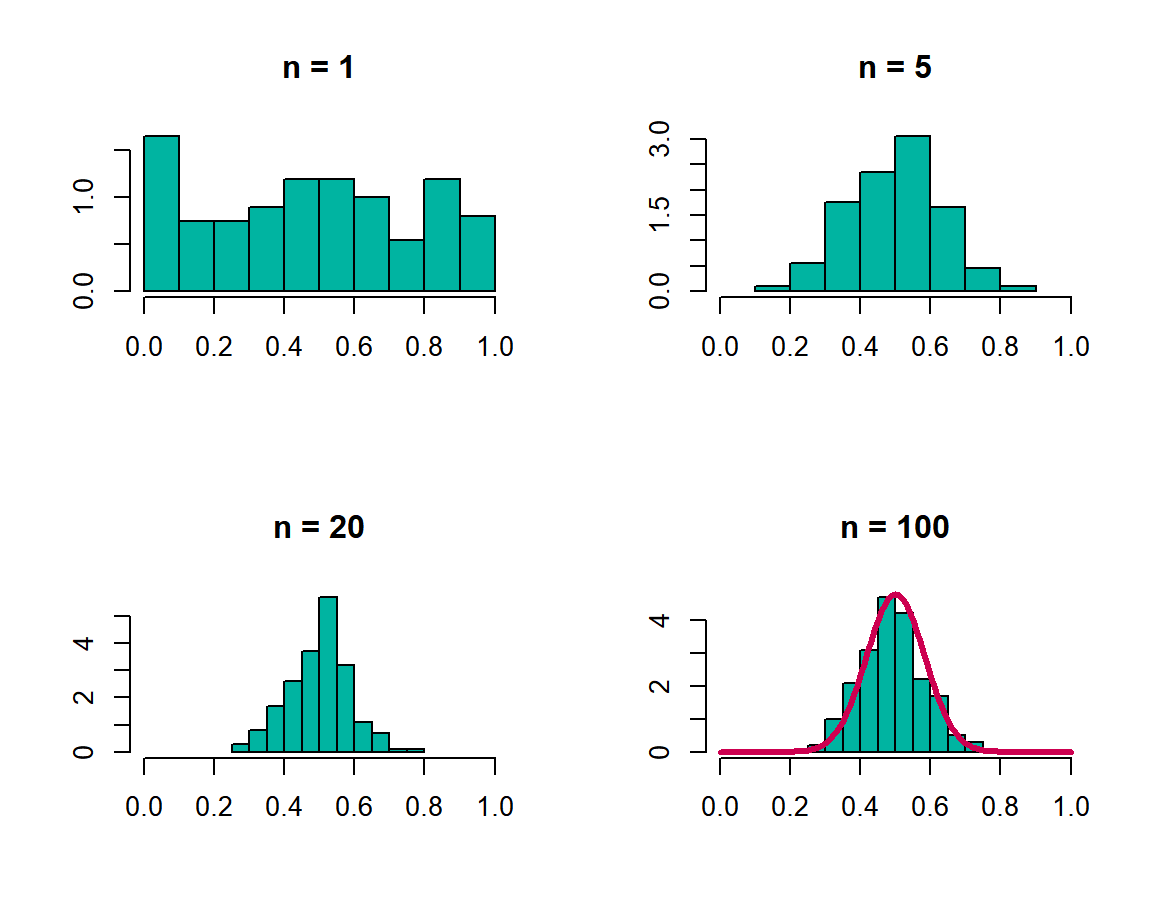
\includegraphics[width=0.7\linewidth]{Statistique_infentielle_files/figure-latex/illust-1} 

}

\caption{Illustration du théorème central limite: histogramme de la moyenne de 200 échantillons issus d'une loi uniforme sur l'intervalle (0,1) en fonction de la taille $n$ de l'échantillon.}\label{fig:illust}
\end{figure}

Les retombées pratiques de ces résultats sont importantes. En effet, la
moyenne de variables aléatoires est une quantité qui intervient dans plusieurs
procédures statistiques. Aussi, le résultat du théorème central limite permet
l'approximation des probabilités liées à des sommes de variables aléatoires (e.g.~méthode de Monte-Carlo).
De plus, lorsque l'on considère des modèles statistiques, le terme d'erreur représente la somme de beaucoup d'erreurs (erreurs de mesure, variables non
considérées, etc.). En prenant comme justification le théorème central limite,
ce terme d'erreur est souvent supposé se comporter comme une loi normale.

\hypertarget{loi-faible-des-grands-nombres}{%
\subsection{Loi faible des grands nombres}\label{loi-faible-des-grands-nombres}}

\BeginKnitrBlock{theorem}[Loi faible des grands nombres]
\protect\hypertarget{thm:fable}{}{\label{thm:fable} \iffalse (Loi faible des grands nombres) \fi{} }Soit \(X_1,\ldots,X_n\) une suite de variables aléatoires indépendantes et identiquement distribuées. On suppose que \(E(|X_i|) < \infty\) et que tous les \(X_i\) admettent la même espérance \(E(X_i)= \mu\). Pour tout \(\epsilon >0\)

\[ \lim_{n \to \infty} P(|\overline{X}_n - \mu|> \epsilon) = 0,\]

c'est-à-dire \(\overline{X}_n\) converge en probabilité vers \(\mu\).
\EndKnitrBlock{theorem}

\hypertarget{loi-forte-des-grands-nombres}{%
\subsection{Loi forte des grands nombres}\label{loi-forte-des-grands-nombres}}

\BeginKnitrBlock{theorem}[Loi forte des grands nombres]
\protect\hypertarget{thm:forte}{}{\label{thm:forte} \iffalse (Loi forte des grands nombres) \fi{} }Soit \(X_1,\ldots,X_n\) une suite de variables aléatoires indépendantes et identiquement distribuées. On suppose que \(E(|X_i|) < \infty\) et que tous les \(X_i\) admettent la même espérance \(E(X_i)= \mu\). Pour tout \(\epsilon >0\)

\[ P\big( \lim_{n \to \infty} \overline{X}_n = \mu \big) = 1 \]

On dit que \(\overline{X}_n\) converge presque sûrement vers \(\mu\).
\EndKnitrBlock{theorem}

\hypertarget{theoreme-central-limite}{%
\subsection{Théorème central limite}\label{theoreme-central-limite}}

\BeginKnitrBlock{theorem}[Théorème central limite]
\protect\hypertarget{thm:central}{}{\label{thm:central} \iffalse (Théorème central limite) \fi{} }Soit \(X_1,\ldots,X_n\) une suite de variables aléatoires indépendantes et identiquement distribuées, d'espérance \(\mu\) et variance \(\sigma^2\) finie. Alors

\begin{equation} 
\frac{\overline{X}_n - \mu}{ \sigma/\sqrt{n}} \xrightarrow{n \to \infty} \mathcal{N}(0,1)
\label{eq:central}
\end{equation}

en distribution.

On voit bien que, afin que la convergence se fasse, une standardisation est
nécessaire: en effet, on peut voir le rapport dans \eqref{eq:central} comme

\[\frac{\overline{X}_n - \mu}{ \sigma/\sqrt{n}} = \frac{\overline{X}_n - E(\overline{X}_n)}{ \sqrt{var(\overline{X}_n)}}\]
\EndKnitrBlock{theorem}

\BeginKnitrBlock{rmdtip}
\textbf{Notes Historiques}

La loi faible des grands nombres a été établie la première fois par J. Bernoulli
pour le cas particulier d'une variable aléatoire binaire ne prenant que les valeurs 0 ou 1. Le résultat a été publié en 1713.

La loi forte des grands nombres est due au mathématicien E. Borel (1871-
1956), d'où parfois son autre appellation: théorème de Borel.

Le théorème central limite a été formulé pour la première fois par A. de
Moivre en 1733 pour approximer le nombre de ``piles'' dans le jet d'une pièce
de monnaie équilibrée. Ce travail a été un peu oublié jusqu'à ce que P.S. Laplace
ne l'étende à l'approximation d'une loi binomiale par la loi normale dans son
ouvrage \emph{Théorie analytique des probabilités} en 1812. C'est dans les premières
années du \(XX^e\) siècle que A. Lyapounov l'a redéfini en termes généraux et
prouvé avec rigueur.
\EndKnitrBlock{rmdtip}

\hypertarget{estimation-ponctuelle}{%
\chapter{Estimation ponctuelle}\label{estimation-ponctuelle}}

\hypertarget{intervalle-de-confiance}{%
\chapter{Intervalle de confiance}\label{intervalle-de-confiance}}

\hypertarget{tests-dhpotheses}{%
\chapter{Tests d'hpothèses}\label{tests-dhpotheses}}

\hypertarget{appendix-annexe}{%
\appendix \addcontentsline{toc}{chapter}{\appendixname}}


\hypertarget{tab:normale}{%
\chapter{Table de la loi Normale centrée réduite}\label{tab:normale}}

\begin{center}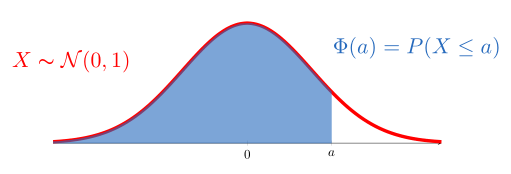
\includegraphics[width=0.7\linewidth]{img/tableau} \end{center}

0

0.01

0.02

0.03

0.04

0.05

0.06

0.07

0.08

0.09

0

0.5000

0.5040

0.5080

0.5120

0.5160

0.5199

0.5239

0.5279

0.5319

0.5359

0.1

0.5398

0.5438

0.5478

0.5517

0.5557

0.5596

0.5636

0.5675

0.5714

0.5753

0.2

0.5793

0.5832

0.5871

0.5910

0.5948

0.5987

0.6026

0.6064

0.6103

0.6141

0.3

0.6179

0.6217

0.6255

0.6293

0.6331

0.6368

0.6406

0.6443

0.6480

0.6517

0.4

0.6554

0.6591

0.6628

0.6664

0.6700

0.6736

0.6772

0.6808

0.6844

0.6879

0.5

0.6915

0.6950

0.6985

0.7019

0.7054

0.7088

0.7123

0.7157

0.7190

0.7224

0.6

0.7257

0.7291

0.7324

0.7357

0.7389

0.7422

0.7454

0.7486

0.7517

0.7549

0.7

0.7580

0.7611

0.7642

0.7673

0.7704

0.7734

0.7764

0.7794

0.7823

0.7852

0.8

0.7881

0.7910

0.7939

0.7967

0.7995

0.8023

0.8051

0.8078

0.8106

0.8133

0.9

0.8159

0.8186

0.8212

0.8238

0.8264

0.8289

0.8315

0.8340

0.8365

0.8389

1

0.8413

0.8438

0.8461

0.8485

0.8508

0.8531

0.8554

0.8577

0.8599

0.8621

1.1

0.8643

0.8665

0.8686

0.8708

0.8729

0.8749

0.8770

0.8790

0.8810

0.8830

1.2

0.8849

0.8869

0.8888

0.8907

0.8925

0.8944

0.8962

0.8980

0.8997

0.9015

1.3

0.9032

0.9049

0.9066

0.9082

0.9099

0.9115

0.9131

0.9147

0.9162

0.9177

1.4

0.9192

0.9207

0.9222

0.9236

0.9251

0.9265

0.9279

0.9292

0.9306

0.9319

1.5

0.9332

0.9345

0.9357

0.9370

0.9382

0.9394

0.9406

0.9418

0.9429

0.9441

1.6

0.9452

0.9463

0.9474

0.9484

0.9495

0.9505

0.9515

0.9525

0.9535

0.9545

1.7

0.9554

0.9564

0.9573

0.9582

0.9591

0.9599

0.9608

0.9616

0.9625

0.9633

1.8

0.9641

0.9649

0.9656

0.9664

0.9671

0.9678

0.9686

0.9693

0.9699

0.9706

1.9

0.9713

0.9719

0.9726

0.9732

0.9738

0.9744

0.9750

0.9756

0.9761

0.9767

2

0.9772

0.9778

0.9783

0.9788

0.9793

0.9798

0.9803

0.9808

0.9812

0.9817

2.1

0.9821

0.9826

0.9830

0.9834

0.9838

0.9842

0.9846

0.9850

0.9854

0.9857

2.2

0.9861

0.9864

0.9868

0.9871

0.9875

0.9878

0.9881

0.9884

0.9887

0.9890

2.3

0.9893

0.9896

0.9898

0.9901

0.9904

0.9906

0.9909

0.9911

0.9913

0.9916

2.4

0.9918

0.9920

0.9922

0.9925

0.9927

0.9929

0.9931

0.9932

0.9934

0.9936

2.5

0.9938

0.9940

0.9941

0.9943

0.9945

0.9946

0.9948

0.9949

0.9951

0.9952

2.6

0.9953

0.9955

0.9956

0.9957

0.9959

0.9960

0.9961

0.9962

0.9963

0.9964

2.7

0.9965

0.9966

0.9967

0.9968

0.9969

0.9970

0.9971

0.9972

0.9973

0.9974

2.8

0.9974

0.9975

0.9976

0.9977

0.9977

0.9978

0.9979

0.9979

0.9980

0.9981

2.9

0.9981

0.9982

0.9982

0.9983

0.9984

0.9984

0.9985

0.9985

0.9986

0.9986

3

0.9987

0.9987

0.9987

0.9988

0.9988

0.9989

0.9989

0.9989

0.9990

0.9990

Par exemple, pour \(x = 1.23\) (intersection de la ligne
1.2 et de la colonne
0.03), on obtient : \(\Phi(1.23) \approx 0.8907\).

\begin{center}\href{https://mghassany.shinyapps.io/shiny_pnorm/}{\includegraphics[width=1\linewidth]{Statistique_infentielle_files/figure-latex/shiny_pnorm-1} }\end{center}

\bibliography{biblio.bib}


\end{document}
